\section{Laser-Cluster interaction}

\subsection{Clusters of atoms and strong laser fields}

Clusters of atoms have been in use for a longer time than we might normally
think. Gold clusters were already used in ancient Rome for their optical
properties; their size could be controlled to produce different glass colours.
Gustav Mie was the first to theoretically describe the interaction of light
with (gold) spheres in 1908, explaining the light absorption dependence
on cluster size. During the last part of the twentieth century, the discovery of
C$_{60}$ fullerenes marked the real beginning of cluster studies\cite{Reinhard2004}.

As the Roman saw, the size of these nanoparticles is a key property. Techniques to fully
control the size of produced clusters allowed a wide range of studies and
applications. Three main class of cluster creation techniques
exists\cite{Reinhard2004}. First, supersonic jets methods force high pressure
gas through a small nozzle into a vacuum chamber where atoms condensate into
clusters. Second, gas aggregation methods similarly condensate atoms after
their injection into a gas chamber. Lastly, clusters can be created by breaking
up a material surface by either particle collision, laser ablation or high
electric field. These techniques gives great control over the created cluster
size.

Along with the recent developments and advances in the nanosciences,
the advance of high-power and short duration lasers opened the
door for ground breaking ultra-fast studies. With femtosecond
(1 fs = 10$^{-15}$ s) lasers it became possible to study electron motion,
similarly to a camera flash that captures a moving scene.


The study of the interaction of rare gas clusters with femtosecond lasers represents a
merging of nano and ultrafast science.
%
Many femtosecond lasers
have a wavelength of 800 nm in the infrared (IR) and cluster have been studied
thoroughly with this ``long'' wavelength. Investigation of energetic
electrons (keV) or highly charged ions (MeV) emission, X-rays production or even
table-top neutron sources\cite{Krainov2007} were performed since the
1990s\cite{Haberland1994,Brabec2009}.


The IR regime sparked a new field of ultrafast physics. By stripping electrons
from their parent ion through tunnel ionization and accelerating them in the
laser's strong electric field, train of pulses of high harmonics can be created,
a process called High Harmonic Generation (HHG).
Created during a single femtosecond pulse, this train of smaller pulses
can reach the attosecond \mbox{(1 as = 10$^{-18}$ s)} duration, an exciting
developing field\cite{Levesque2006}.


Clusters are invaluable tools because they bridge the gap between single atoms
and solids. Their high density allows them to exhibit collective effects similarly
to bulk materials while their small
size increases their surface to volume ratio.
At the smallest range, clusters can be used as models for small molecules and
at the opposite they still present interesting optical properties even at 10,000
atoms\cite{Reinhard2004}.

Additionally to their great size scalability, clusters explosion by-products
after interaction with a strong laser field are accessible, revealing detailed
information about the dynamics. For example, time-of-flight (TOF) mass
spectrometry can reveal the ions charge state spectrum which
is a signature of the amount
of energy absorbed from the laser pulse. This kind of data is not accessible
in the case of laser-bulk interaction since the majority of matter stays
in the solid.

Clusters of atoms can be composed of different elements. Rare gas atoms have
closed outer electronic shells which makes them less prone to chemical
reactions and so don't interact much with each other. Rare-gas clusters are
thus weakly bound by Van der Waals forces and generally form
an icosahedral structure\cite{Martin1996}. The electronic wavefunctions are
more localized around the nucleus than in metal clusters which simplifies the
treatment of the cluster environment.

A critical characteristic of laser-cluster interaction for the present
work is the fact that clusters can be studied numerically. Full quantum resolution
is not possible even for clusters consisting of a couple of atoms, while on the
other range of the methods spectrum rates equations and (nano)plasma models are
too macroscopic to reflect the large fields gradient present during cluster
dynamics\cite{Fennel2010}. The tool of choice for this problem is Molecular Dynamics
(MD) where dynamics are treated classically; Newton's equations of motion are
solved at each time steps and quantum effects are included using specific rates.

The importance of laser-cluster interaction as an investigative tool
can be seen by the vast amount of work on the subject, mainly
in the IR regime\cite{Fennel2010}. Varin \textit{et al.}\cite{Varin2012}
recently developed an electrodynamic
particle-in-cell (PIC) code for IR studies on pre-ionized clusters. PIC methods
have a better scaling than MD in terms of particles number and since they treat
the electromagnetic field dynamically (through Maxwell's equations) field
retardation effects are taken into account, which can be important for large
clusters. On the down side PIC methods don't have the precision of MD for close
range interactions and collisions. A novel addition by Varin \textit{et al.}
is to add microscopic corrections to PIC for more realistic close range
interactions\cite{Peltz2012}.
Since the grid must resolve the electromagnetic wave,
PIC simulations can thus be a challenge when the wavelength is small
but this opens the door to a new frontier of modelling.

The interest of this thesis is in modelling short wavelength interaction with
clusters. In recent years, laser light sources have been moving to shorter
wavelengths due to groundbreaking new Free Electron Lasers (FEL)
facilities; Vacuum Ultra-Violet (VUV), Extreme Ultra-Violet (XUV), soft X-Rays
and even hard X-rays are now accessible. In FELs, relativistic electrons are sent
through an ondulator in which they emit a coherent pulse, tunable in wavelength
(by changing the electrons initial energy)
from microwaves to X-rays\cite{Brabec2009,Ackermann2007a,Pellegrini2012} at
unprecedented intensities. A single 10 to 100 fs FEL pulse can contain 10$^{13}$
photons, the same amount produced by the best synchrotrons during
\textit{one second}\cite{Bostedt2009}. Even though FEL installations require
large facilities, some researchers are working on a smaller version, as
``short'' as 55 meters\cite{Shintake2008}.

% http://ieeexplore.ieee.org/stamp/stamp.jsp?tp=&arnumber=5500378
At shorter wavelengths, treating the laser as simply an electromagnetic field
during ionization is not valid anymore and photons must be considered instead.
The Keldysh parameter $\gamma$ dictates which ionization regime must be considered. In
cases where $\gamma \ll 1$ the electric field of the laser is strong enough that
the ion's Coulomb potential is distorted to such an extent
that electrons can tunnel out.
However, when $\gamma \gg 1$ the laser frequency is too large compared to the
field's strength. Ionization is then dominated by single (or a few) photon
absorption.
Experiments in
2002\cite{Wabnitz2002,Bostedt2009} at
DESY's FLASH (\textbf{F}ree-electron-\textbf{Las}er in \textbf{H}amburg)
on Xenon clusters in the VUV regime (98~nm wavelength, 12.65~eV photon energy)
had $\gamma$ values between 8 and
100 putting it in the regime dominated by photon processes.
During these experiments, unexpected high charge states were seen that could not
be explained by traditional energy transfer mechanisms. Theoretical work was
then performed for explaining these high charge states; these models will be
covered in section \ref{section:intro:mechanisms}.



At shorter wavelength,
Argon clusters were studied in the XUV regime\cite{Bostedt2008}. The 32.8~nm
(37.8~eV) photons are 5 eV above Argon's first ionization
potential. It was found that ionization is a multistep process of
photo-electrons emission and because of the subsequent charge buildup in the
cluster, the electron energy distribution is non-thermal.

In 2006, a proof-of-principle experiment showed that that it is possible to
do (soft) X-rays diffraction imaging using FLASH pulses\cite{Chapman2006}:
Chapman \textit{et al.} were able to image a micrometer-wide stick-figure pattern
engraved on a 20 nm thin film. Imaging was possible even though the sample was
eventually destroyed by the high intensity X-ray laser pulse.
Similar studies on Xenon clusters were performed in 2010\cite{Bostedt2010} where
diffraction patterns where obtained for clusters in single laser shots
at 13 nm (95.37 eV).

More multiphoton
ionization experiments on Nitrogen, Argon, Neon and Helium were performed at
FLASH.
% [8] A.A. Sorokin et al., “Multi-photon ionization of molecular nitrogen by femtosecond soft X-ray FEL pulses,” J. Phys. B: At. Mol. Opt.
% Phys. 39, L299-L304 (2006).
% [9] A. Fohlisch et al., “High-brilliance free-electron-laser photoionization of N2: Ground-state depletion and radiation-field-induced modifi-
% cations”, Phys. Rev. A 76, 013411 (2007).
% [10] R. Moshammer et al., “Few-Photon Multiple Ionization of Ne and Ar by Strong Free-Electron-Laser Pulses,” Phys. Rev. Lett. 98,
% 203001 (2007).
% [11] A. Rudenko et al., “Recoil-Ion Momentum Distributions for Two-Photon Double Ionization of He and Ne by 44 eV Free-Electron
% Laser Radiation,” Phys. Rev. Lett. 101, 073003 (2008).
% [12] A.A. Sorokin et al., “X-ray-laser interaction with matter and the role of multiphoton ionization: Free-electron-laser studies on neon and
% helium” Phys. Rev. A 75, 051402(R) (2007).
% [13] M. Nagasano et al., “Resonant two-photon absorption of extreme-ultraviolet free-electron-laser radiation in helium,” Phys. Rev. A 75,
% 051406(R) (2007).
At the even shorter wavelength of 13.7 nm (90.5~eV), Xenon clusters irradiated at
$\ten{7.5}{15}$~W/cm$^2$ produced charged states of up to 21+\cite{Sorokin2007,Richter2009},
meaning 60 XUV photons had to be absorbed per atom. Xenon's giant 4d
resonance is suspected to be the cause of these high charge states.

The Linac Coherent Light Source (LCLS) at SLAC, Stanford, is another important
FEL facility where the first FEL hard X-rays lasing was
performed in 2010\cite{Emma2010,Schneider2010}. Single Neon atoms were studied in
this hard X-rays source\cite{Young2010} showing fully stripped neon nucleus.
Later, protein nanocrystallography was performed
on photosystem~I in 2011\cite{Chapman2011} and on photosystem~II in
2013\cite{Kern2013}. These two large cell membrane proteins are implicated in
photosynthesis of algae, plants, and some bacteria.
By using pulses shorter
than the explosion time scale, the protein's structure could be reconstructed,
opening the door for the determination of the structure of biomolecules that
do not crystallize correctly for use in traditional crystallography studies.
In the same Nature issue, Mimivirus, the second largest known virus at 450 nm
of diameter, was imaged using single shot hard X-ray pulse (0.69~nm,
1.8~keV)\cite{Seibert2011}. LCLS pulses have a duration of 70 to 500 fs at
wavelengths of 0.15 nm to 2.2 nm\cite{Pellegrini2011}.

Cluster studies continue to this day in regimes such as VUV\cite{Arbeiter2011},
XUV\cite{Murphy2008a,Murphy2008b,Krikunova2012} and X-rays\cite{Ziaja2009b,Thomas2012,Timneanu2013}
and there is much theoretical work to be done as new phenomena are uncovered.

% http://photon-science.desy.de/facilities/flash/publications/selected_publications/index_eng.html
% https://portal.slac.stanford.edu/sites/lcls_public/Pages/Publications.aspx


\subsection{Microscopic mechanisms underlying cluster dynamics}
\label{section:intro:mechanisms}

Interaction of light with single rare gas atoms is a well studied problem but
the collective effects of the high density of atoms in a cluster gives rise to
many different mechanisms of energy absorption and redistribution throughout the
cluster. This section will cover the different mechanisms by going over the
different wavelength regimes, from the long wavelength (IR) to the shorter XUV.

The different mechanisms described in this section can be sorted into two main
families. First, the laser-driven, or laser-particles, mechanisms are the
simplest as they are the result of the direct interaction between the laser
and the particles. They are normally described using isolated atoms but can
be adapted to take into consideration the cluster environment; see section
\ref{section:intro:Vb} for details. For example, single-photon ionization where
one photon is absorbed by a bound electron and gets promoted to the continuum is
a direct interaction between the laser and the atom.

The second family consist of indirect mechanisms were particles-particles
interaction are vital. These indirect mechanisms don't necessarily transfer
energy from the laser to the cluster but are still an important aspect of
cluster dynamics as they can affect energy absorption and charge state spectra.
For example, impact ionization where
an electron hits an atom and promotes a bound electron to the continuum by
sharing some of its kinetic energy is independent on the presence of a laser
(but obviously still requires free electrons). As will be described later,
indirect mechanisms are still important for the cluster dynamics and can also
help energy transfer from the laser to the cluster.

The cluster environment, due to the large particle density, has an important
influence on both the laser-driven and particles-particles interaction and
aspects of how to incorporate its effect on laser-cluster interaction
is a substantial aspect of the current work.

Most studies on clusters are performed on femtosecond IR laser
pulses which span a large range of intensity. These kind of lasers are
widespread and dominated by Ti:sapphire pumped with another laser. The pump
laser (Nd:YAG) lases at 1064 nm and is frequency-doubled to 534 nm in a
nonlinear crystal. The Ti:sapphire then emits 800 nm light with a wide range of
intensity.

The advance of Free-Electron Lasers (FEL) allowed high intensity of VUV, XUV and
even X-rays laser source. As described previously, FEL require large facilities,
mainly due to the linear particle accelerator required to seed the ondulator
with relativistic electrons and as such are scarce and their intensity is limited
compared to Ti:sapphire lasers. Nevertheless their
tunable wavelength allows them to access different interesting regimes.

The different regimes are shown on figure \ref{fig:regimes}.
The vertical axis shows the different regimes as
function of wavelengths. They will be presented, in the following subsection,
in order of wavelength, from longest to shortest. At each regime, dominant
processes will be presented.

% http://www.spacewx.com/Docs/ISO_PRF_21348_e_review.pdf
As can be seen on figure \ref{fig:regimes}, the laser's intensity also dictates
the regime.
The Keldysh adiabatic parameter $\gamma$ separates regimes where ionization
processes are dominated by either photons or field\cite{Long2010} and reads
\begin{align}
% http://www.iuac.res.in/atmol/~safvan/safvan_thesis/node32.html
\gamma & = \sqrt{ \frac{\textrm{Ip}}{2 U_p} } = \frac{\omega}{\omega_t},
\end{align}
where Ip is the atom's ionization potential, $U_p$ is the ponderomotive energy
\begin{align}
% https://en.wikipedia.org/wiki/Ponderomotive_energy
U_p & = \frac{e^2 E^2}{4 m \omega^2},
\end{align}
$e$ and $m$ the electron's charge and mass, $E$ the laser's electric field
strength, $\omega$ its angular frequency and $\omega_t$ the tunnelling
frequency:
\begin{align}
\omega_t & = \frac{e E}{\sqrt{2 m \textrm{Ip}}}
\end{align}

When $\gamma~\ll~1$, the laser field strength is large compared to the ionization
potential. In that case, a bound electron will feel a significant bending of the
atomic potential and will thus have a significant probability of tunnelling out.
For this to happen, the ionization potential Ip must be
smaller than the ponderomotive energy $U_p$. Figure \ref{fig:regimes} shows,
as dashed lines, constant values of the ponderomotive energy. The plain line shows
a ponderomotive energy value equal to the (first) ionization potential of Xenon.
The field dominated regime lies under this line.

Otherwise, when $\gamma~\gg~1$, the laser field strength is weak compared to
the ionization potential and the later is not as important as before in the
subsequent dynamics. The amplitude of the electron's quiver motion in the laser
field is given by
\begin{align}
% Georgescu2007a, page 3
x_q & = \frac{F}{\omega^2}
\label{eqn:quiver}
\end{align}
where $F$ is the force of the laser field and $\omega$ its angular frequency.
When $\gamma~\gg~1$, the quiver amplitude $x_q$ is minimum; the electric field
oscillates too rapidly for the electrons to feel it and photon interactions with
the cluster is thus dominant.

Note that the two regimes are not clearly segregated; Keldysh parameter
predicts which process will dominate -- photon processes or field processes --
but both can occur. Photon processes could happen in the field-dominated
regime and the laser field can still move electrons around in the photon-dominated regime.

\begin{figure}
\centering
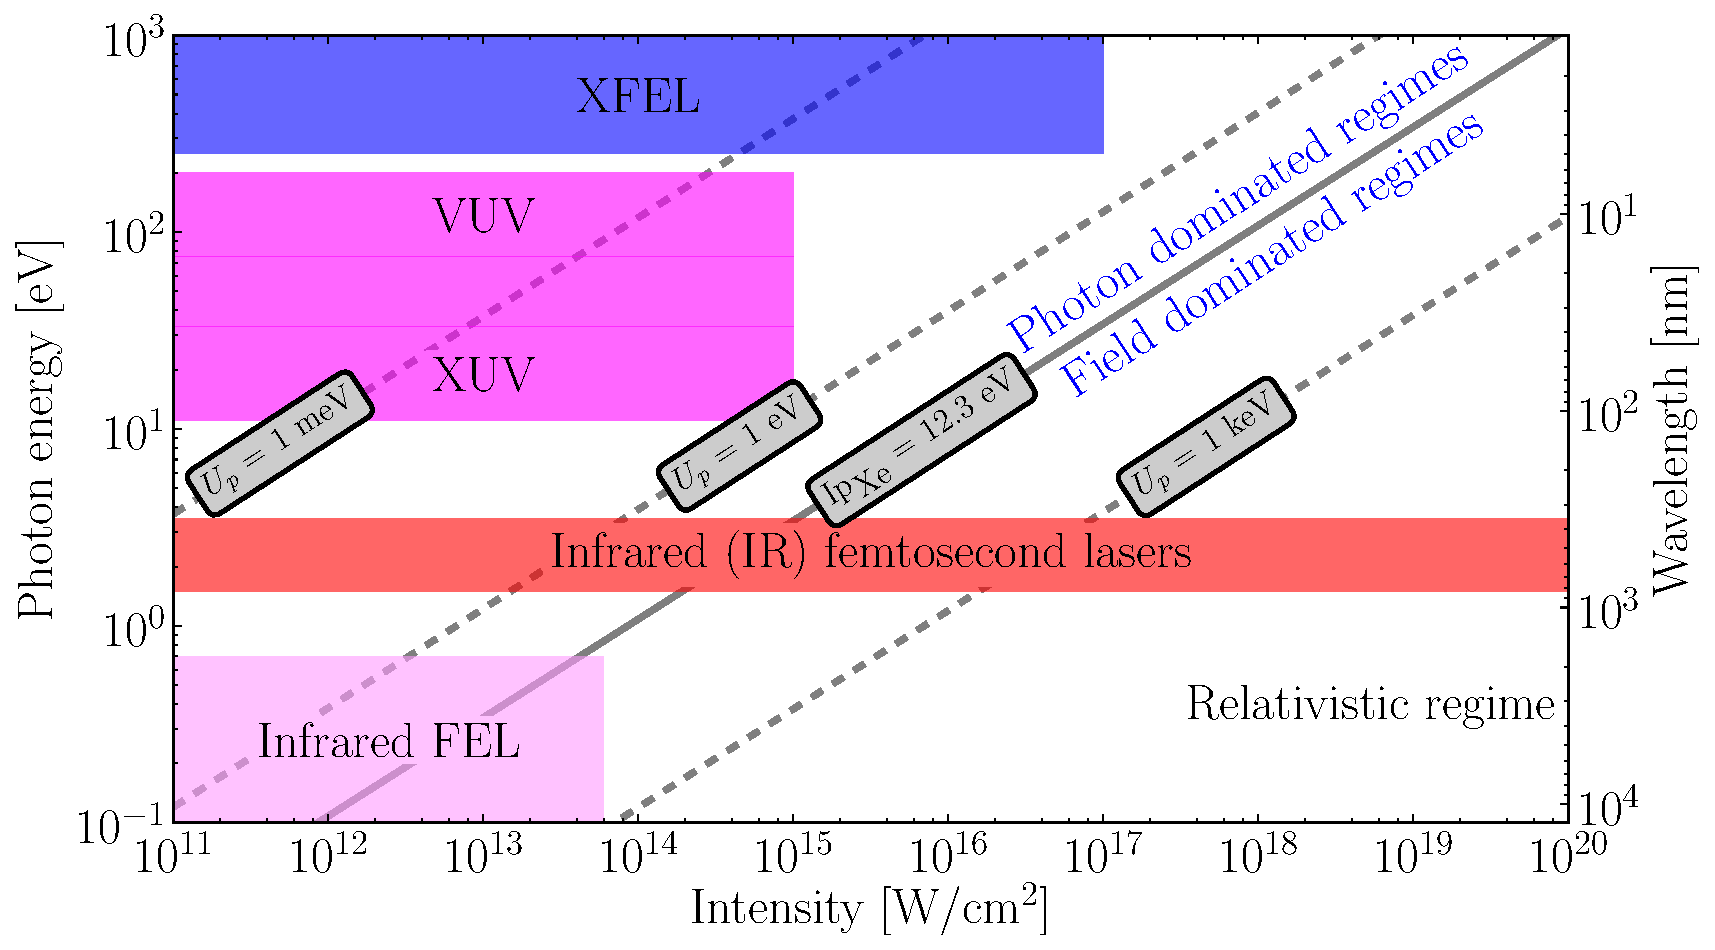
\includegraphics[width=\figurewidth]{figures/regimes}
\caption{Wavelength and intensity regimes. For Xenon, lower right half is dominated
         by field processes while upper left half by photon processes. Diagonal
         lines represent constant ponderomotive potential $U_p$. The
         demarcation between the two halves happens when the ponderomotive
         potential equals the ionization potential ($U_p = Ip$).
         Note that the present work concentrate on the VUV and XUV regimes
         where photon processes dominates (at the studied intensities).}
\label{fig:regimes}
\end{figure}

In table \ref{tab:ips} the first ionization energies for the different
rare gas elements used in this thesis (Argon and Xenon) are shown. As can be
seen from the table and figure \ref{fig:regimes}, Xenon and Argon can be
single-photon ionized in the VUV regime where photons of 15.76 (for Argon)
and 12.13 eV (for Xenon) are possible. While Xenon's 5p states have the smallest
Ip's, the cross-section for photoionization of the 4d shell is approximately ten
times larger at 13.7 nm (90.5 eV) -- the so called xenon giant 4d
resonance\cite{Becker1986} -- making ionization of these inner-shells
possible\cite{Thomas2009,Ackad2013}.
% http://photon-science.desy.de/news__events/research_highlights/archive/flash_excites_giant_atomic_resonance/index_eng.html

\begin{table}
\begin{center}
\begin{tabular}{cccccc} \hline
\mc{3}{c}{Argon} & \mc{3}{c}{Xenon} \\
Configuration
        & Ip [eV]
                    &$\lambda$ [nm]
                                & Configuration
                                        & Ip [eV]
                                                    & $\lambda$ [nm] \\ \hline
% Used in the code:
% 16.00   & 77.49             & 12.265625 & 101.1 \\
% 32.34   & 38.34             & 21.390625 & 57.96 \\
% 48.68   & 25.47             & 31.296875 & 39.62 \\
% 65.02   & 19.07             & 41.859375 & 29.62 \\
% 81.56   & 15.20             & 55.015625 & 22.54 \\ \hline
%
% Experimental data (from NIST):
% http://physics.nist.gov/PhysRefData/ASD/levels_form.html
3p$^5$  & 15.7596109& 78.6721   & 5p$^6$& 12.129843 & 102.214 \\
3p$^4$  & 27.62967  & 44.8736   & 5p$^5$& 20.975    & 56.4 \\
3p$^3$  & 40.735    & 30.4368   & 5p$^4$& 31.05     & 39.9305 \\
3p$^2$  & 59.58     & 20.8097   & 5p$^3$& 42.20     & 29.3801 \\
3p$^1$  & 74.84     & 16.5666   & 5p$^2$& 54.1      & 22.9176\\
3s$^2$  & 91.290    & 13.5814   & 5p$^1$& 66.703    & 18.5875 \\
3s$^1$  & 124.41    & 9.96577   & 5s$^2$& 91.6      & 13.5354 \\
 &  &   & 4d$^{10}$ & 105.978   & 11.699 \\
 &  &   & 4d$^{9}$  & 179.84    & 6.89414 \\
 &  &   & 4d$^{8}$  & 202.0     & 6.13783 \\
 &  &   & 4d$^{7}$  & 229.02    & 5.41368 \\
 &  &   & 4d$^{6}$  & 255.0     & 4.86213 \\
 &  &   & 4d$^{5}$  & 280.9     & 4.41382 \\
 &  &   & 4d$^{4}$  & 314.1     & 3.94728 \\
 &  &   & 4d$^{3}$  & 342.9     & 3.61575 \\
 &  &   & 4d$^{2}$  & 374.1     & 3.3142 \\
 &  &   & 4d$^{1}$  & 403.9     & 3.06968 \\ \hline
\end{tabular}
\caption{First few ionization potentials for (atomic) rare gas elements.
         Source: NIST\cite{NIST}}
\label{tab:ips}
\end{center}
\end{table}

Let us now turn to a more detailed examination of the different mechanisms
present in the different regimes, as well as some regime-independent processes.



\subsubsection{Long wavelength: The IR regime}
\label{section:intro:mechanisms:ir}

Most femtosecond lasers are Ti:sapphire that have a wavelength centred around 800 nm.
This type of lasers sparked the research on clusters. They cover a wide range of
intensity and as such can touch different regimes, from the photon-dominated
one at low intensities to the field-dominated one at larger intensities and
even going up to where relativistic effects cannot be neglected.

One can see how much work was done in the field-dominated (IR) regime over the
years by looking at the wide literature on the subject, see for example ref.
\cite{Fennel2010} or \cite{Ramunno2008}. On the opposite, the VUV and XUV regime
-- the photon-dominated one -- is much less explored and is thus the main
aspect of the present work. Some effects in the IR are still presented here
for clarity. These processes are dominant in the field-dominated regime (see
figure \ref{fig:regimes}).


\subsubsubsection{Above Threshold Ionization (ATI)}

Above Threshold Ionization (ATI) was one of the first observed effects of
intense laser-matter interaction in 1979\cite{Agostini1979}.
In ATI, more photons are absorbed by atoms
than is normally required to ionize it. This results in photoelectrons spectra
showing peaks at energies much larger than expected separated by the photon
energy. Because its a multiphoton process, ATI requires large
intensities~($\gamma \ll 1$)\cite{Krainov1997,Lewenstein2008}.


\subsubsubsection{Tunnel ionization}

The most striking effect in the IR regime is tunnel
ionization\cite[Chapter~3]{Brabec2009} when intensity reaches 10$^{14}$~W/cm$^2$.
The Coulomb potential of an atom can be bent enough by the (oscillating) laser
field and the probability of a bound electron tunnelling out becomes significant,
as shown on figure \ref{fig:ionization:tunnel}. Tunnel ionization is also
sometimes called optical field ionization (OFI), or more simply field
ionization, since one can describe the process as the laser field as the source
of the potential bending and ionization.
\lrnote{I made the change to the last sentence, but
am still not happy with it. it's b/c the laser field picture is really only a
semiclassical quantum picture in the length gauge. i will clarify more when we
talk and maybe we can edit it appropriately then.}


% Above Threshold Ionization (ATI) https://en.wikipedia.org/wiki/Above_Threshold_Ionization_%28ATI%29
% Strong Field Approximation (SFI)
% http://massey.dur.ac.uk/resources/cpchirila/
\begin{figure}
 \centering
 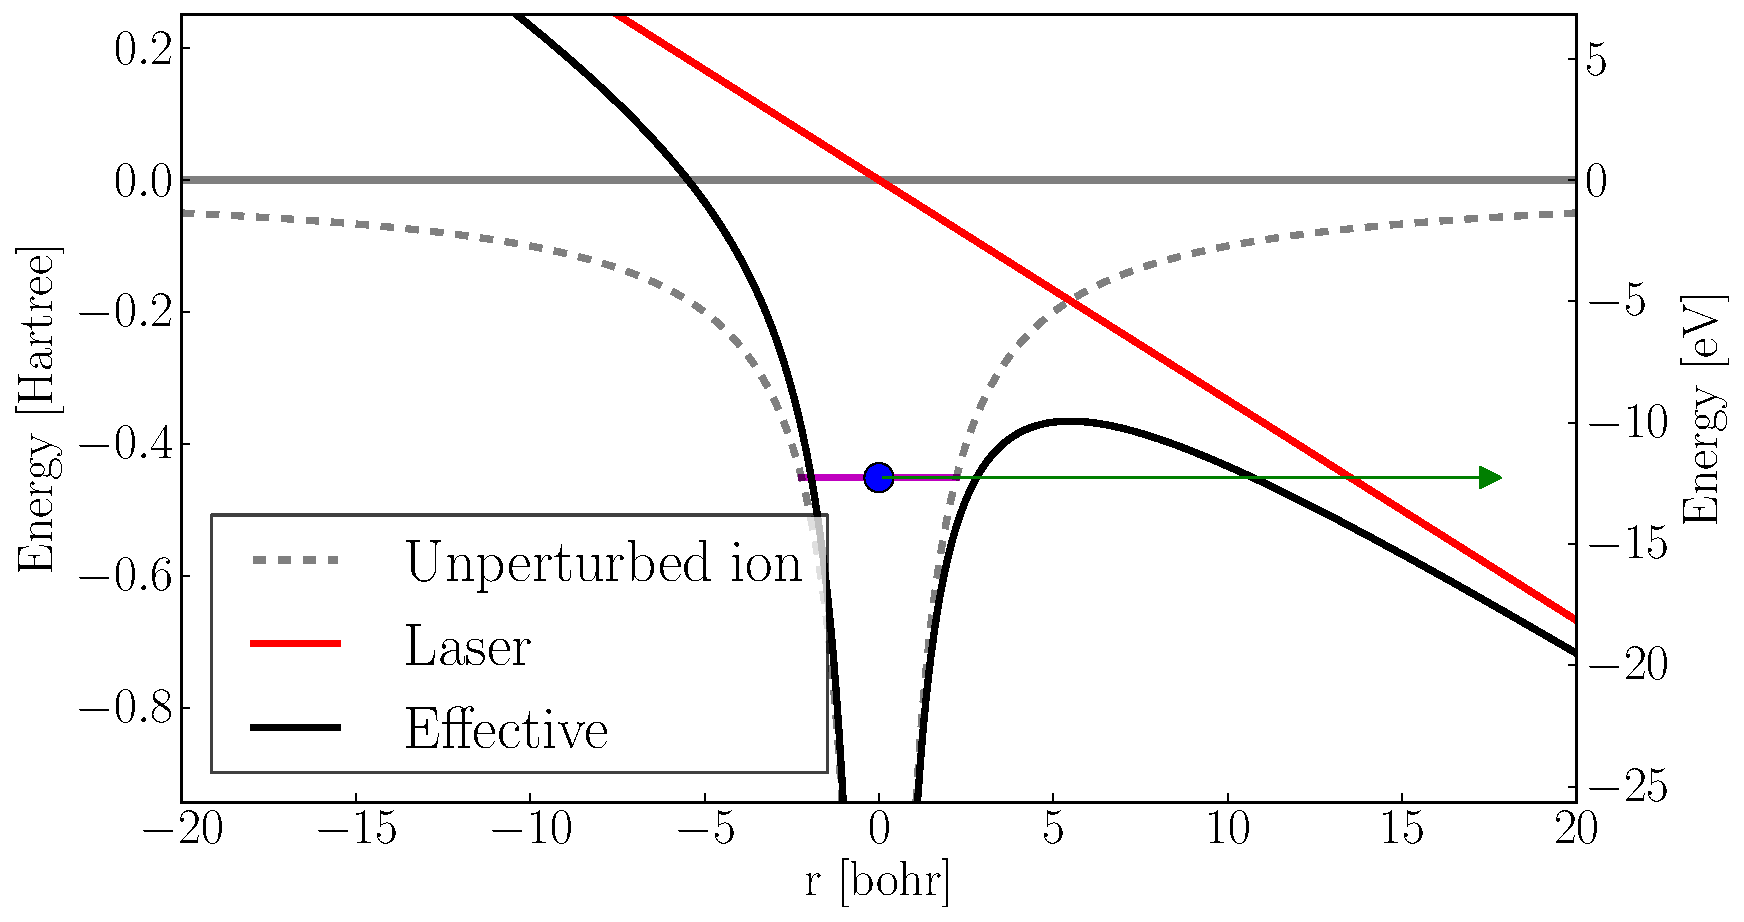
\includegraphics[width=\figurewidth]{figures/ionization_tunnel}
 \caption{\label{fig:ionization:tunnel}Tunnel ionization. The potential
          due to the laser (red) bends the unperturbed ion potential
          (grey dashed). The electron (blue dot) sitting at the unperturbed
          eigenvalue (magenta) now has a probability to tunnel through the total
          potential barrier (black line). The laser frequency must be small
          enough for the probability to be non-negligible (large wavelength)
          and intensity large enough ($\gamma \ll 1$).}
\end{figure}

Tunnel ionization is at the heart of High Harmonic Generation (HHG) and
attosecond science\cite{Fennel2010}. A laser pulse, normally in the IR regime,
bends the atomic potential bounds electrons are feeling, allowing them to tunnel
out. They are then accelerated in the laser field where they gain energy.
As the laser field changes direction within a laser cycle, electrons are forced
back onto their parent ion where they can
recombine and emit high energy photons. The emission spectra,
containing only odd harmonics, shows an intensity decrease as a function of
harmonic number, followed by a plateau and a cutoff. Since the description
of the phenomena in 1993\cite{Corkum1993}, HHG studies expended into its own
sub-field. For example, Murphy \textit{et al.} used the 21st harmonic of a
800 nm Ti:sapphire to ionize xenon clusters\cite{Murphy2008a,Murphy2008b}
with these new 32.6 eV (38 nm) photons.
For more details on HHG see references~\cite{Levesque2006} and
\cite{Lewenstein2008}.
\lrnote[noinline,margin]{you should be prepared to answer "why only odd harmonics?"}


\subsubsubsection{Inverse Bremsstrahlung Heating}

Once electrons are created in the IR regime they can continue to absorb energy
from the laser.
Inverse Bremsstrahlung Heating (IBH) is the inverse process of Bremsstrahlung
where an electron emits a photon when deflected, either by a heavier ion in the
case of plasma, or by magnetic fields in the case of synchrotrons. IBH is thus
the absorption of photons accelerating the electrons\cite{Schlessinger1979}.

For large frequencies, the quiver amplitude of equation \eqref{eqn:quiver} is
small; the electric field oscillates
too rapidly for the electrons to gain significant acceleration. On the other
hand, for smaller frequencies (larger wavelengths) the quiver amplitude can
be significant. In the case of IR, electrons can be pushed outside the cluster
and back in; at $\ten{3}{16}$~W/cm$^2$ and 800~nm, the quiver
amplitude is $x_q \approx 500 a_0$, where $a_0$ is the Bohr
radius\cite{Georgescu2007}, while a Xe$_{1415}$ cluster is~115~$a_0$.

The linear momentum gained by electrons in the laser field is then redistributed
as thermal energy by collisions and scattering on heavier ions.
IBH plays an important role in the IR regime where the laser field easily
drives the electrons through the cluster\cite{Fennel2010}.


The IBH rate is given\cite{Fennel2010} by:
\begin{align}
\left< \dt{E} \right> & = 2 U_p \frac{\tau \omega^2}{\tau^2 \omega^2 + 1}
\end{align}
where $\tau$ is the inverse of the collision electron-ion frequency.

\fxfatal{According to Bostedt2010\cite[page 3]{Bostedt2010}, IBH scales as
$\lambda^{8/3}$ and cites Krainov2000\cite{Krainov2000} and
Krainov2002\cite{Krainov2002}}
% ? can you explain the problem to me when we talk next?

\subsubsection{Shorter wavelengths: Into the VUV and XUV regime}
\label{section:intro:mechanisms:vuv}

% http://www.laserfocusworld.com/blogs/what-the-hecht/2012/05/euv-xuv-acronym.html
% http://www.spacewx.com/Docs/ISO_PRF_21348_e_review.pdf
% http://www.iso.org/iso/home/store/catalogue_tc/catalogue_detail.htm?csnumber=39911

With the help of new FEL facilities, high laser intensities can be reached at
lower wavelength (and thus larger photon energy) than with traditional
femtosecond lasers. \textit{Vacuum ultraviolet} (VUV) radiation, ranging from 200 to
10~nm (6.2 to 124~eV), is normally absorbed by the atmosphere. Studying them
requires vacuum chambers (hence the name) or a pure nitrogen propagation medium.
At short wavelengths, the photons can start to ionize inner shell electrons. In
that case, the term \textit{extreme ultraviolet} (XUV, or EUV) is used. XUV wavelengths
range from 121~nm (hydrogen's Lyman alpha line, 10.25 eV) to 10~nm (124~eV).
As the two regimes have overlapping wavelengths, they are often used
interchangeably but XUV is generally used with wavelengths where no
material is known to be transparent\cite{Laane2009}. Note that in other fields
XUV can be used to describe soft X-rays\cite{Eichmeier2008,iso21348}

At relatively low intensity (less than 10$^{14}$~W/cm$^2$
\cite{Ramunno2008}), in the photon-dominated regime, atoms and ions
can be ionized by photon absorption. If the photon energy is more than the
electron's biding energy (see table \ref{tab:ips} for numerical values) single
photon ionization will be the dominant energy transfer mechanism.

While not as strong as in the IR regime, IBH is still important in the
VUV\cite{Krainov2000} up to 62 nm\cite{Georgescu2007}.


\subsubsubsection{Photon absorption}

Initially described by Einstein as the photoelectric effect, a bound electron
absorbs a photon from the laser and is promoted to the continuum where it is
free to leave its parent ion. Figure~\ref{fig:ionization:single} shows a
schematic of the mechanism. For example, the first energy level of atomic
Xenon is at -12.27 eV requiring a photon wavelength equal or shorter than
101.1 nm for ionization.


\begin{figure}
 \centering
 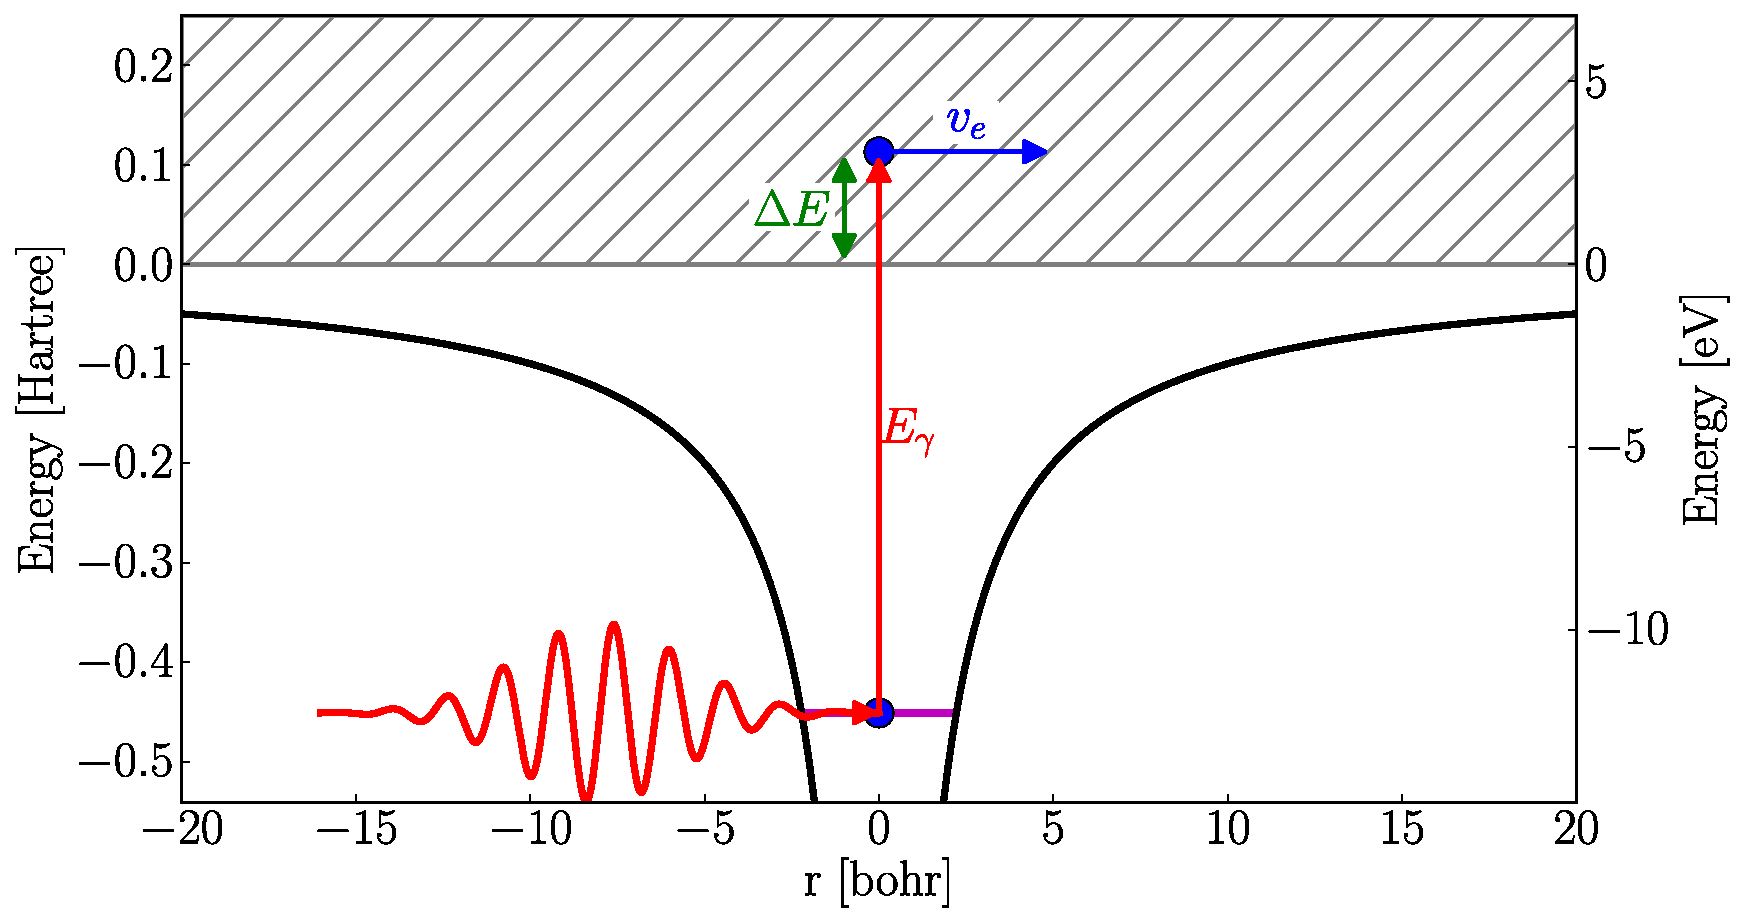
\includegraphics[width=\figurewidth]{figures/ionization_single}
 \caption{Single photon ionization for the atomic, isolated model. A photon
          (red) is absorbed by a bound electron (blue) which gets promoted to
          the continuum. The remaining energy $\Delta E$ between the photon's
          and the Ip results in electron's kinetic energy $K_e$.
          Chapter \ref{section:tools} describes the cluster environment
          influence.}
 \label{fig:ionization:single}
\end{figure}

If the photon energy exceed the electron's binding energy, the difference in energy
will be transferred as extra kinetic energy in the
resulting photoelectron. This can thus be used to sample the states in the
target by measuring the photoelectron energy spectrum\cite{Fennel2010}.

However, if the photon energy is less then the binding energy, than a single
photon cannot ionize an atom. If the intensity is large enough though, the
photon density will be sufficient that many photons can be absorbed during a
small time interval.
This effect is called multiple-photon ionization (MPI, not to
be confused with the Message Passing Interface used in parallel programming) and
is a non-linear process. The ionization rate of $\nu$-photons MPI is given
by\cite{Fennel2010}:
\begin{align}
\Gamma_{\nu} = \sigma_{\nu} I^{\nu}.
\label{eqn:ionization:rate:mpi}
\end{align}
Being a nonlinear process, multi photon ionization is present at larger
intensities than single photon ionization. But being photon processes, both are
superseded by tunnel ionization at even larger intensities (or when
$\gamma~\gg~1$).

\lrfatal[noinline,margin]{there is also the above-threshold ionization
regime, which you might want to mention, and was one of the first discoveries in
the atto field}

% \clearpage
\subsubsubsection{Auger effect}

At even shorter wavelength, the photon energy might be large enough not only
to ionize the highest energy electron but also some inner-shell electrons.
When such an inner shell electron gets ionized, it leaves a hole; the atom is
thus in an excited state. An outer shell electron will then transition by
\textit{Auger decay} to the hole. The transition energy is used by a third
electron (the Auger electron) to leave the ion, leaving the latter
doubly-ionized. Figure \ref{fig:auger} shows a diagram of the process.

\begin{figure}
 \centering
    \begin{subfigure}{0.48\columnwidth}
        \centering
        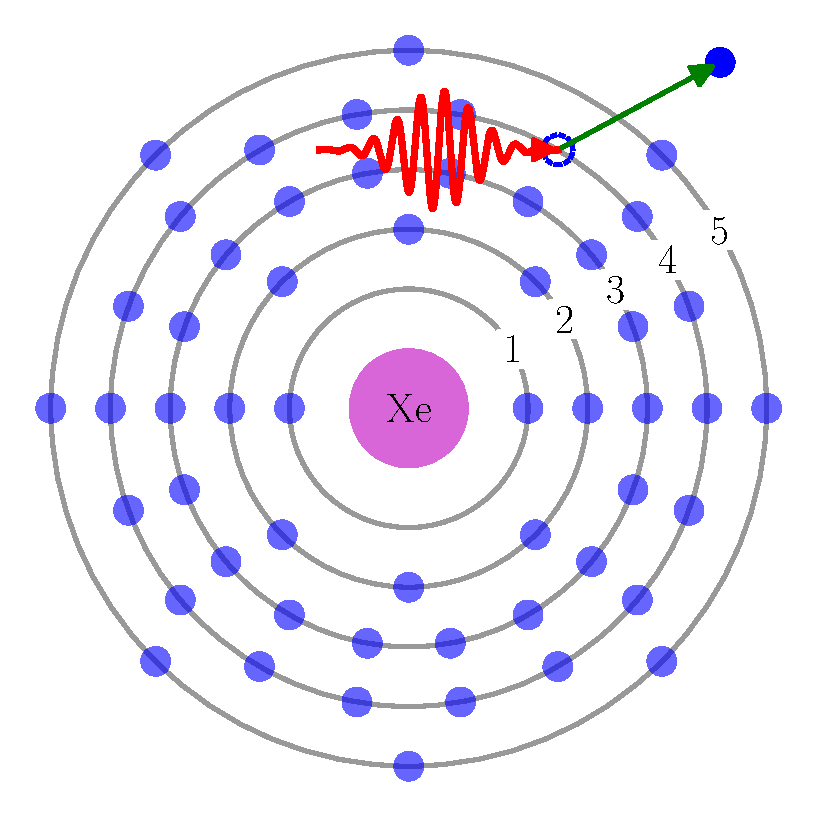
\includegraphics[width=\textwidth]{figures/auger_step_1}
        \caption{Step 1: An xenon 4d inner shell electron absorbs a high
                 energetic photon and leaves the atom. \\}
        \label{fig:auger:1}
    \end{subfigure}
    \begin{subfigure}{0.48\columnwidth}
        \centering
        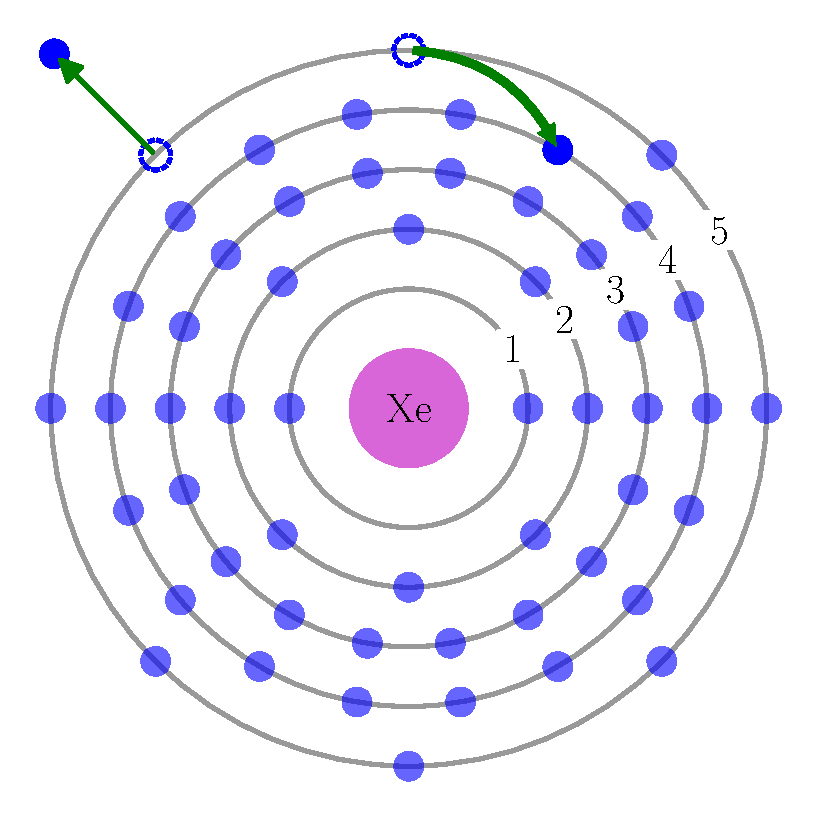
\includegraphics[width=\textwidth]{figures/auger_step_2}
        \caption{Step 2: An outer shell electron decays into the created hole,
                 transferring the energy difference between the two states to a
                 third electron which is ejected (the Auger electron).}
        \label{fig:auger:2}
    \end{subfigure}
        \caption{\label{fig:auger}Auger ionization of a xenon 4d electron by a
                 high energetic X-ray photon. Xenon's 54 electrons are shown
                 as blue dots with the distance to the core representing their
                 principal quantum numbers $n$.}
\end{figure}

To access core electrons, photons must be highly energetic, normally in X-rays.
While not the focus of the present work, an interesting aspect is that Xenon
atoms have a giant resonance of the (inner-shell) 4d state; the cross-section of
photoionization of the 4d electron is ten times larger than the
one of valence  electrons at 13.7 nm wavelength~(90.5~eV)\cite{Becker1986}.
This process was included in the model for a comparison with a 2009 experiment
by Thomas \textit{et al.}\cite{Thomas2009} on Xenon clusters at FLASH-DESY.
The German group saw clusters becoming nanoplasmas from which the outer shells
ions undergo Coulomb explosion while the relatively neutral core expands
hydrodynamically. These results could be reproduced by our model in a recently
published article entitled ``Recombination effects in soft-x-ray cluster
interactions at the xenon giant resonance'', published in May 2013 in
\textit{New Journal of Physics}\cite{Ackad2013} and included in section
\ref{section:papers:recomb}.

% ******************************************************************************
\subsubsection{Regime independent processes}
\label{section:intro:mechanisms:noregime}

Once electrons are created in the cluster, other mechanisms appear. During
impact ionization a first electron collides with an atom and, if it has enough
kinetic energy, will transfer a portion of it to a bound electron, promoting it
to the continuum. Figure \ref{fig:ionization:impact} shows the energy diagram
of the process.

\begin{figure}
 \centering
 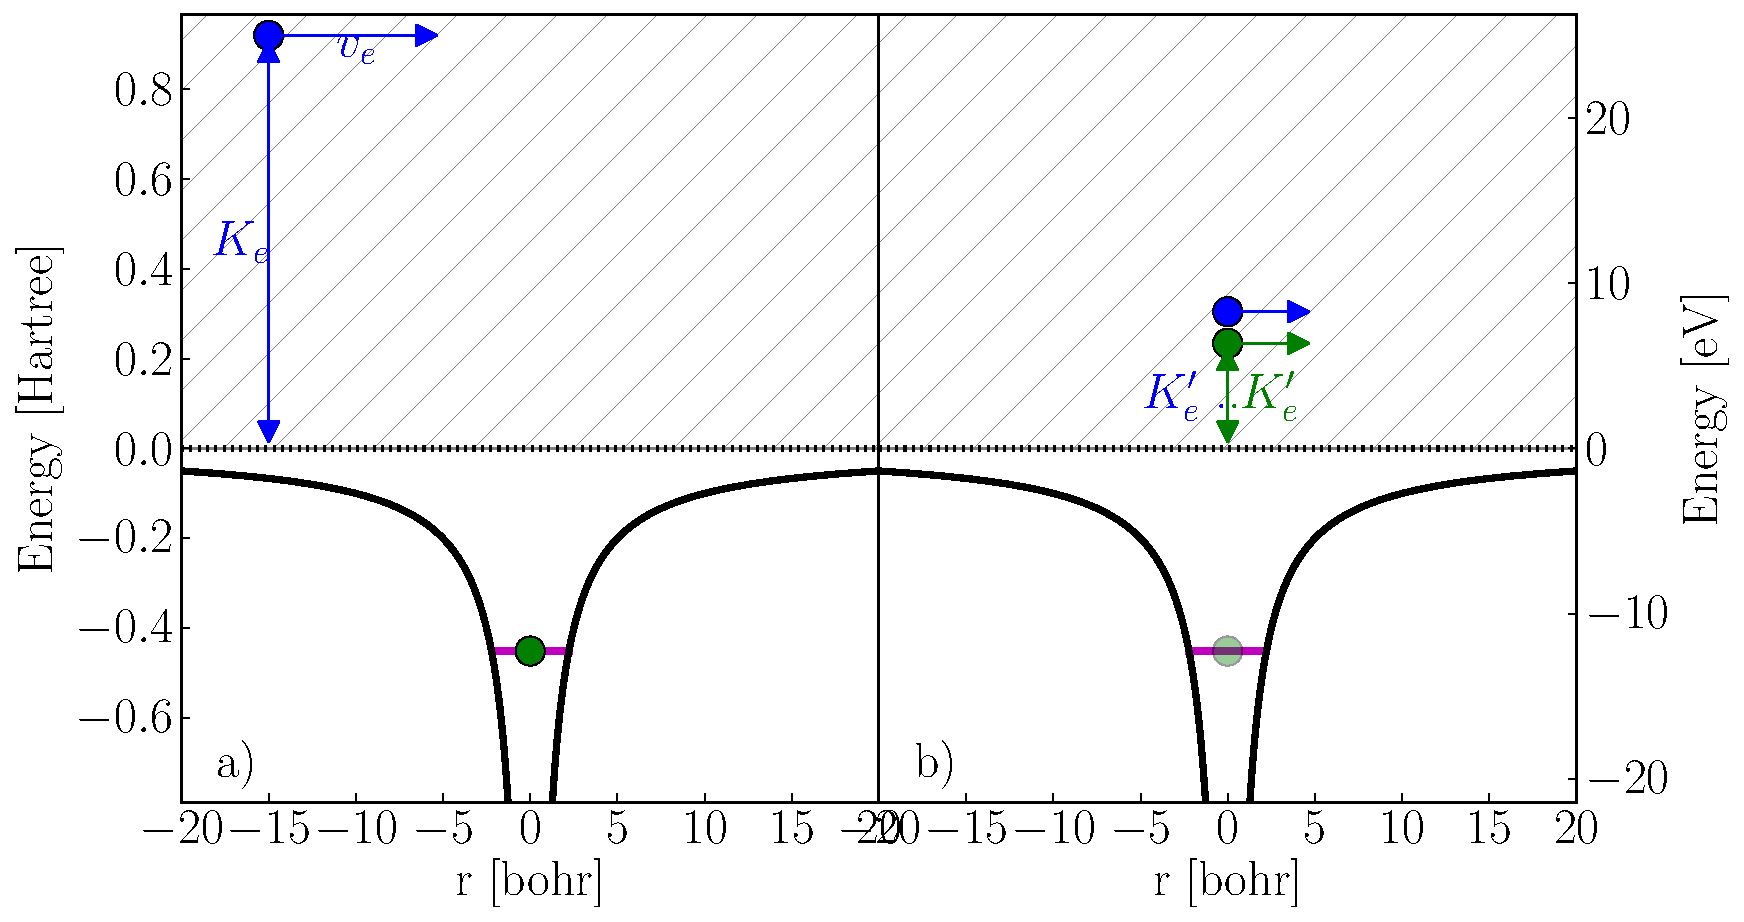
\includegraphics[width=\figurewidth]{figures/ionization_impact}
 \caption{Impact ionization. The colliding electron (blue dot) gives a portion
          of its energy to a bound electron (green dot), promoting it to the
          continuum.}
 \label{fig:ionization:impact}
\end{figure}

Impact ionization can be modelled through cross-sections. These
cross-sections are normally obtained from the semi-empirical Lotz
formula\cite{Lotz1967}:
\begin{align}
\sigma & = \sum_{i}^{N} a_i q_i \frac{\ln{\pa{E/\textrm{Ip}_i}}}{E \textrm{Ip}_i} \pa{1 - b_i
\ex{-c_i \pa{E/\textrm{Ip}_i - 1}}}
\label{eqn:impact:ionization:lotz}
\end{align}
where Ip$_i$ is the ionization potential of the $i^{\textrm{th}}$ shell and $E$
the impacting electron's kinetic energy \textit{at infinity} (or above threshold).

\subsubsection{New regime, new processes}
\label{section:intro:mechanisms:new},

By going to shorter wavelengths, FEL installations allowed experiments at high
intensities in the VUV and XUV regime. These experiments saw surprisingly
high charge states as the results of the clusters
explosion\cite{Wabnitz2002,Bostedt2010}. For example, Wabnitz \textit{et al.}
saw, at FEL-DESY, Xe$^{4+}$ when Xe$_{80}$ clusters were irradiated with 98 nm,
100 fs FEL pulses of, what was though at the time, $\ten{2}{13}$~W/cm$^2$
intensity. For larger clusters (Xe$_{30,000}$), Xenon ions up to
Xe$^{8+}$ were observed. This was a big surprise considering that the 98~nm
photons (12.7 eV) could only ionize neutral Xenon to Xe$^{1+}$ by itself;
data showed that up to 30 photons were absorbed per atom for the largest
clusters. Using a different source of photons and at a different wavelength
(21st harmonic of an 800 nm Ti:sapphire, XUV: 32.6 eV, 38 nm),
Murphy \textit{et al.} observed the same pattern of high charge states in xenon
clusters\cite{Murphy2008a,Murphy2008b}.

Such high charge states could not be explained by the previous processes only.
New mechanisms were thus proposed to explain these surprising results.
The four main models proposed throughout the years are covered next.


\subsubsubsection{Atomic potentials}

First, Santra \& Greene proposed using \textit{atomic potentials} instead of
the Coulomb potential in a rate equation model (with infinite spatial
extension and
constant density) as seen on figure \ref{fig:heating:atomic_pot}.
The atomic nucleus is normally shielded by bound electrons but inside the
electronic cloud the shielding disappears and the nucleus potential is more
important. If an impacting electron can get close enough to the core, it will
feel the unshielded potential.
In reference \cite{Greene2003}, Santra \& Greene used an approximated form for
the atomic potential, fitting one parameter with the first ionization potential.
A later\cite{Walters2006} publication used a
potential shape generated by the code written by Herman and
Skillman\cite{HS1963} (HS) to describe a more realistic
potential, based on a
Hartree-Fock formulation. Using these atomic potentials, they saw Xe$^{3+}$,
Xe$^{5+}$ and Xe$^{7+}$ for intensities of $\ten{1.4}{12}$, $\ten{1.4}{13}$ and
$\ten{7.3}{13}$~W/cm$^2$ respectively for Xe$_{1,500}$ clusters, similarly to
what was seen in at FEL-DESY.


\subsubsubsection{Barrier suppression}

Another model proposed by Siedschlag and Rost\cite{Siedschlag2004} in 2004 was
the barrier suppression in single photon absorption which is shown on figure
\ref{fig:heating:barrier}. Due to the close proximity
of neighbours, the potential barrier between them is lowered and
a photo-transition to the continuum becomes possible, even with a single photon.

\lrnote{nic, did we ever talk about the downsides of the rost model?}

\subsubsubsection{Many-Body Recombination}

\textit{Many-Body Recombination} (MBR) was proposed in 2005\cite{Jungreuthmayer2005}
as a simple mechanism to explain the high charge states seen in the
experiments at FEL-DESY. In a strongly coupled plasma, electrons can recombine
easily to a high excited
state after collisions with many bodies. Later, these newly bound electrons can
absorb a new photon from the laser field for another transition to the
continuum -- see figure \ref{fig:heating:mbr}.
Because MBR is much more efficient than three-body
recombination (due to the large density of charged particles), much more
photons are absorbed this way. It was also shown that MBR deposited more energy
in the clusters than traditional IBH.
The simplicity of the
method lies in the fact that in a classical MD simulation, MBR is automatically
included without extra implementation as the high excited states have energies
which are close to each other and can thus be treated classically.
Jungreuthmayer \textit{et al.} were able
to see Xe$^{3+}$, Xe$^{5+}$ and Xe$^{7+}$ for intensities of $\ten{1.5}{12}$,
$\ten{1.5}{13}$ and $\ten{7}{13}$~W/cm$^2$ respectively when simulating
Xe$_{1,000}$ clusters.

\begin{figure}
 \centering
    \begin{subfigure}{0.48\columnwidth}
        \centering
        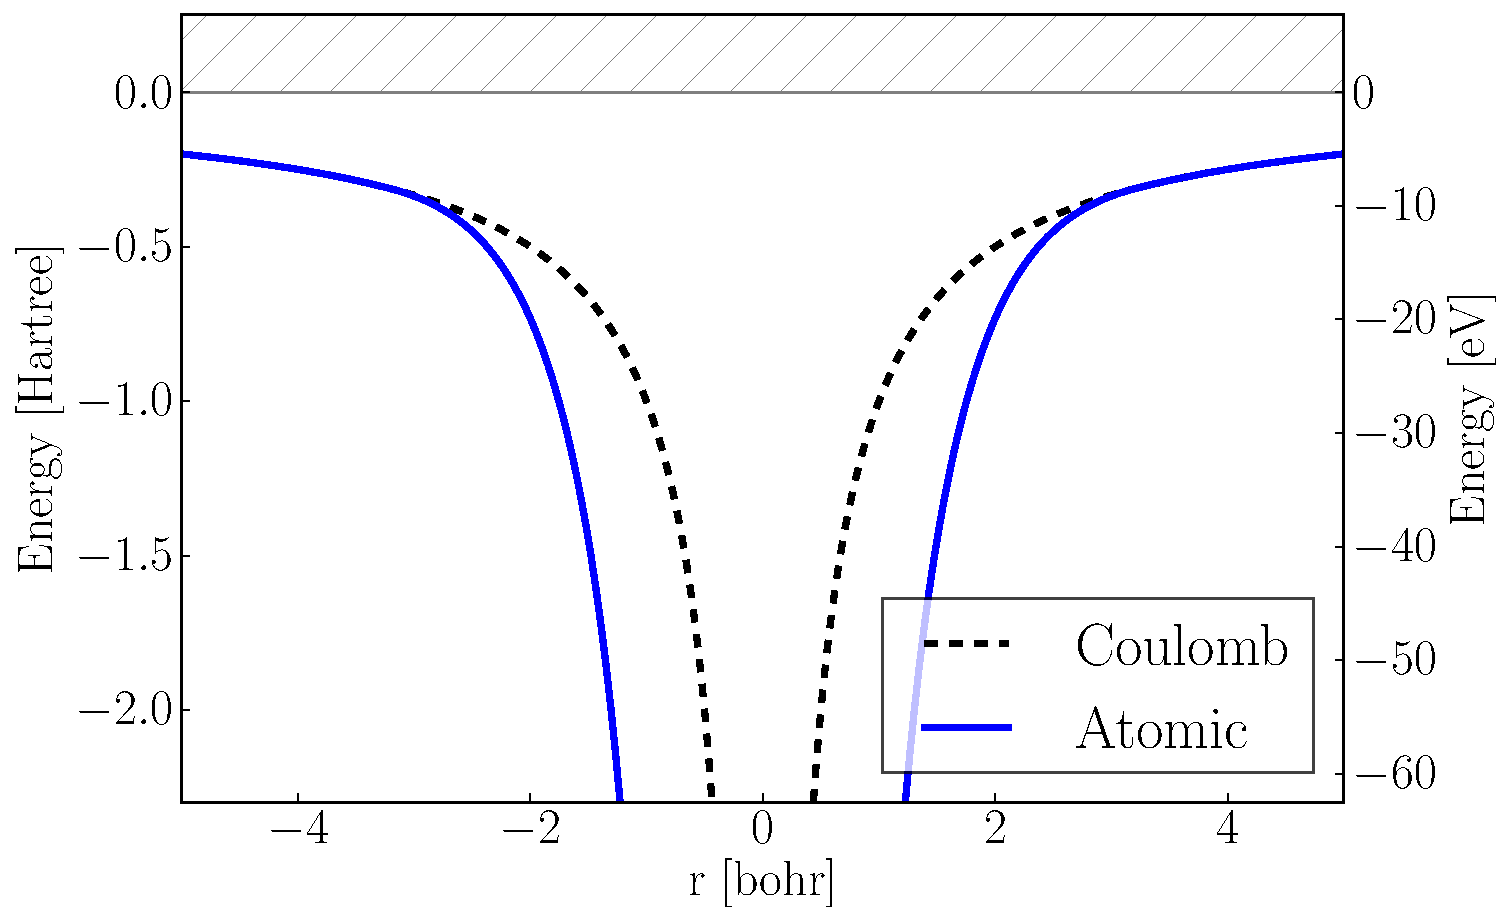
\includegraphics[width=\textwidth]{figures/heating_atomic_potential}
        \caption{Atomic potential (blue line) drops faster than Coulomb one
                (black dashed line), allowing more energy absorption through
                IBH.\\}
        \label{fig:heating:atomic_pot}
    \end{subfigure}
%
    \begin{subfigure}{0.48\columnwidth}
        \centering
        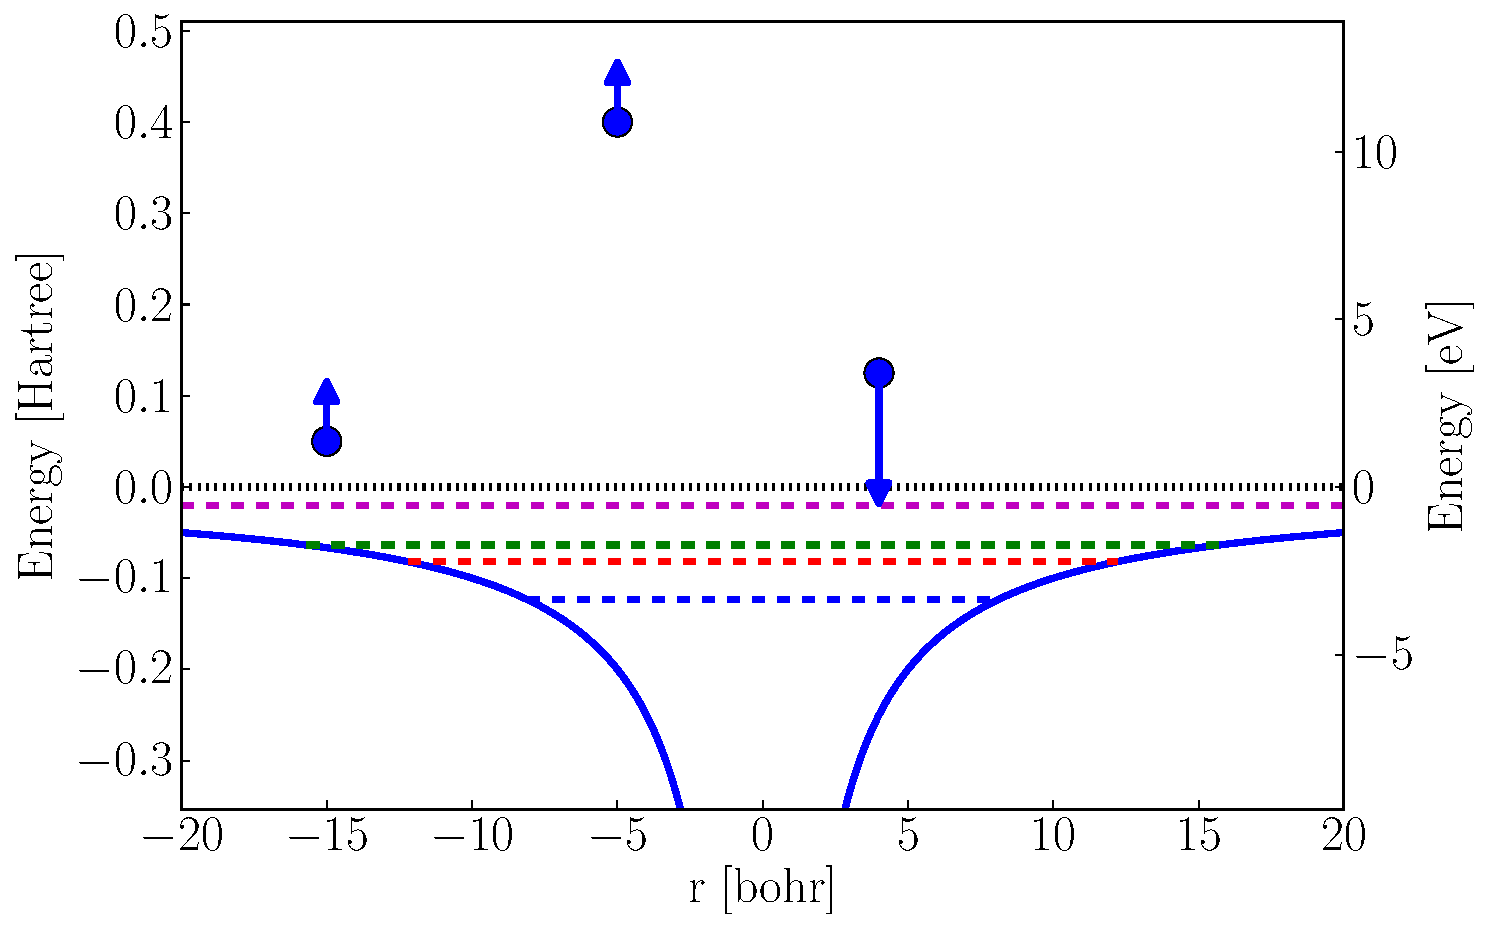
\includegraphics[width=\textwidth]{figures/heating_mbr}
        \caption{MBR: energy exchange between free electrons during collisions
                 makes one recombine to a highly excited state where it can
                 reabsorb a new photon from the laser field.}
        \label{fig:heating:mbr}
    \end{subfigure}
\\
    \begin{subfigure}{\figurewidth}
        \centering
        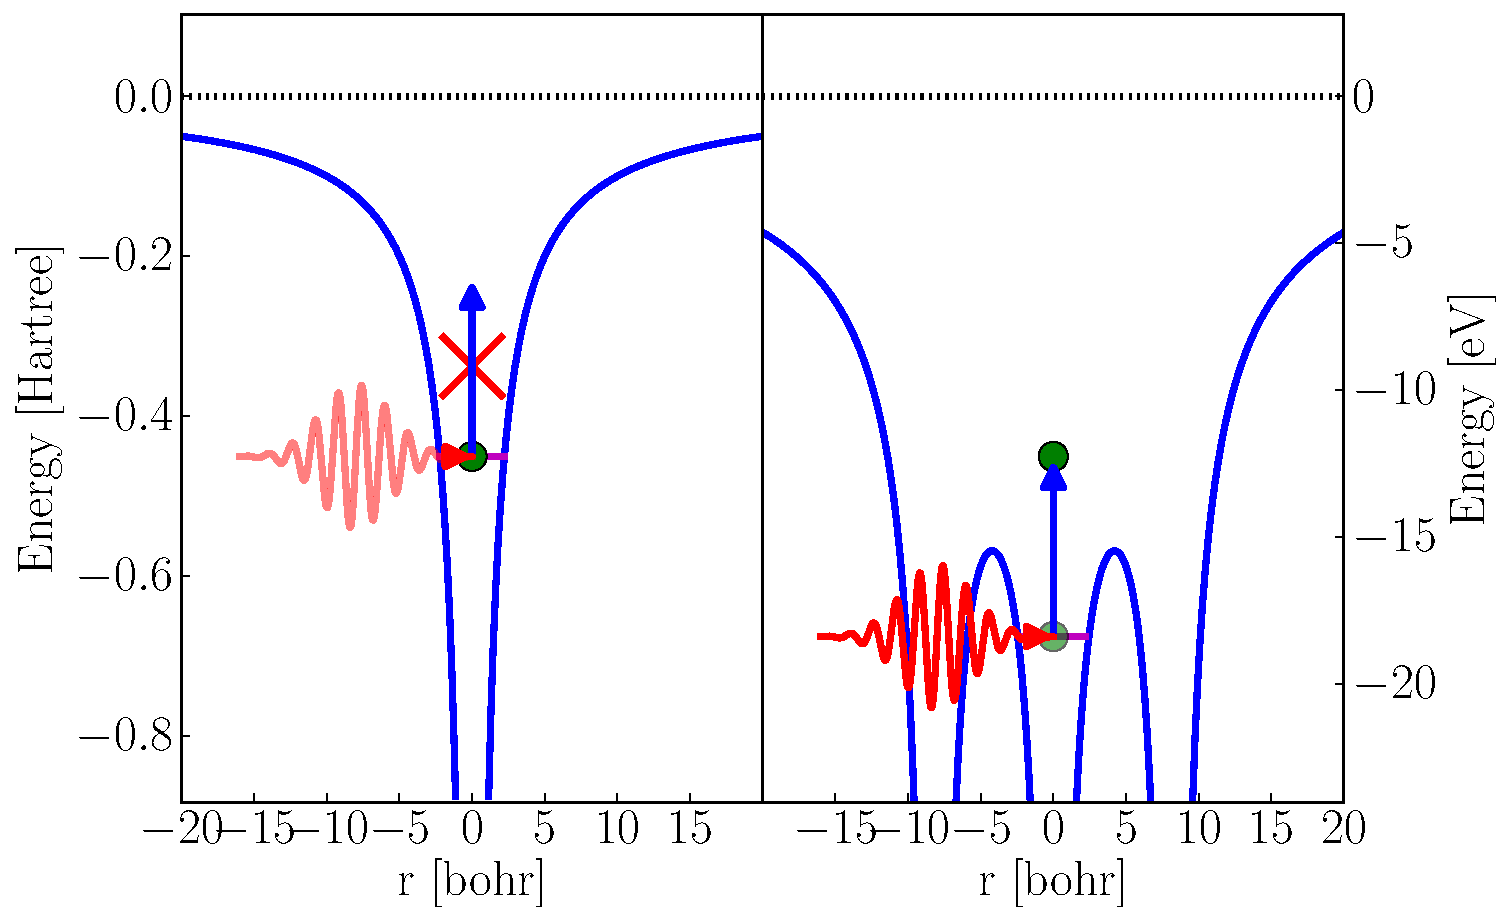
\includegraphics[width=\textwidth]{figures/heating_barrier_sup}
        \caption{Barrier suppression between ions in a cluster environment allows
                 a single photon to ionize deeper levels (right), not accessible
                 with a single atom (left).}
        \label{fig:heating:barrier}
    \end{subfigure}
 \caption{More heating mechanisms}
 \label{fig:heating}
\end{figure}



\clearpage
\subsection{Contributions of thesis}

The goal of the current thesis is to acquire a better understanding of
laser-matter interaction.
More specifically, the
question of \textit{how} the energy is deposited in a nanoscale object
--a rare gas cluster-- by an
ultra-short and ultra-intense laser pulse will be studied. This interaction
largely depends on the specific target material and on the pulse's wavelength
and duration, both defining the interaction regime. A specific regime will
thus be targeted; mainly short wavelengths, from VUV to XUV, as many questions
raising from recent experiments are still debated.

While many tools exist to study laser-mater interaction, only classical
approaches can be considered as a full quantum calculation, even
with some degree of approximations, is not possible. Clusters become
nanoplasmas quite rapidly and have large charge and field fluctuations inside
them. This and their finite nature makes it hard to use tools such as rate
equations to model them. Pure classical simulations allows for relatively large
systems to be simulated and are thus the tool of choice.

\lrnote{also remind me to talk to you about justifications of classical
regmies in plasma physics... we might add that discussion here.}

\subsubsection{Tools}

First, section \ref{section:tools} describes the different tools and models
that were developed and implemented to answer our questions. While section
\ref{section:tools:md} concentrate on the classical aspect of the problem,
section \ref{section:tools:qfdtd} describes in detail a quantum approach that
was used named QFDTD for Quantum Finite-Difference Time-Domain.
Note that all implementations used are original work; all code packages
were developed from scratch by me or under my direction and no external packages
were used. The MD package described in
section \ref{section:tools:md} ($\sim$16k lines of code) contains 86~\% of code
written by me, 12~\% by Edward Ackad (postdoctoral fellow) and smaller contributions from
Julien Roy (undergraduate student) during his summer 2012 internship. Furthermore, the QFDTD package
($\sim$16k lines of code) contains 3~\% of code written by Stan Hatko (undergraduate student) while the
rest is my original work. Most tools were written in C++ with Python being used
for analysis and plotting.

For libraries described in section \ref{section:tools:libraries}, 79~\% of the
ionization library was written by me, 20~\% by Edward Ackad and smaller
contributions from Stan Hatko during his summer 2012 internship. All other
libraries described in section \ref{section:tools:libraries} were fully
written and developed by me.

All these powerful tools were extremely useful for my studies and will also allow
the group to continue its investigation of laser-clusters interaction even
after my departure.

Additionally to the models described in
section \ref{section:intro:mechanisms}, a notable new one was
developed that revealed be of great importance in the description of
laser-clusters interaction. This new model is discussed next.


\subsubsection{Augmented Collisional Ionization (ACI)}

Wabnitz's \textit{et al.} experiments at FLASH-DESY in 2002 revealed the
interestingly high charge states in xenon clusters. Since then, different groups
proposed models to explain these results as described in section
\ref{section:intro:mechanisms:new}.
Then, in 2010, Bosted \textit{et al.}
re-calibrated the intensity used during the 2002 experiments.
Instead of the previously thought $\ten{2}{13}$~W/cm$^2$, the intensity was
re-calibrated to $\ten{8}{12}$~W/cm$^2$, less than half of the initial value.
Could the different models still produce the same amount of high charge states
at the lower intensities?

Additionally, in 2008 experiments \cite{Bostedt2008,Murphy2008b} were performed
in the XUV regime near 30~nm~(41~eV). At this wavelength, the photon energy is
too small for inner shell ionization of rare gas atoms, yet too large
(at reported intensities) for any appreciable laser-field-driven processes, such
as collisional heating, that dominate intense laser-cluster interactions at
longer wavelengths. This presents the opportunity to isolate the influence of
the internal electronic structure from the laser-cluster interaction.

Our group thus proposed a new mechanism for energy transfer from the laser field
to the cluster via two-step collisional ionization. With this two-step model, an
electron might not have enough kinetic energy to directly collisionally ionize
an atom (or ion), but it could still transfer some of
its energy to promote a bound electron to an excited state. Once an atom is
excited, it becomes easier to ionize, due to the large cross-sections of excited
atoms and ions, by subsequent impact from a low energy electron. This gives the
opportunity for low energy electrons to still participate in the cluster
ionization, giving the name \textit{augmented collisional ionization} (ACI) to
the process.

\begin{figure}
 \centering
 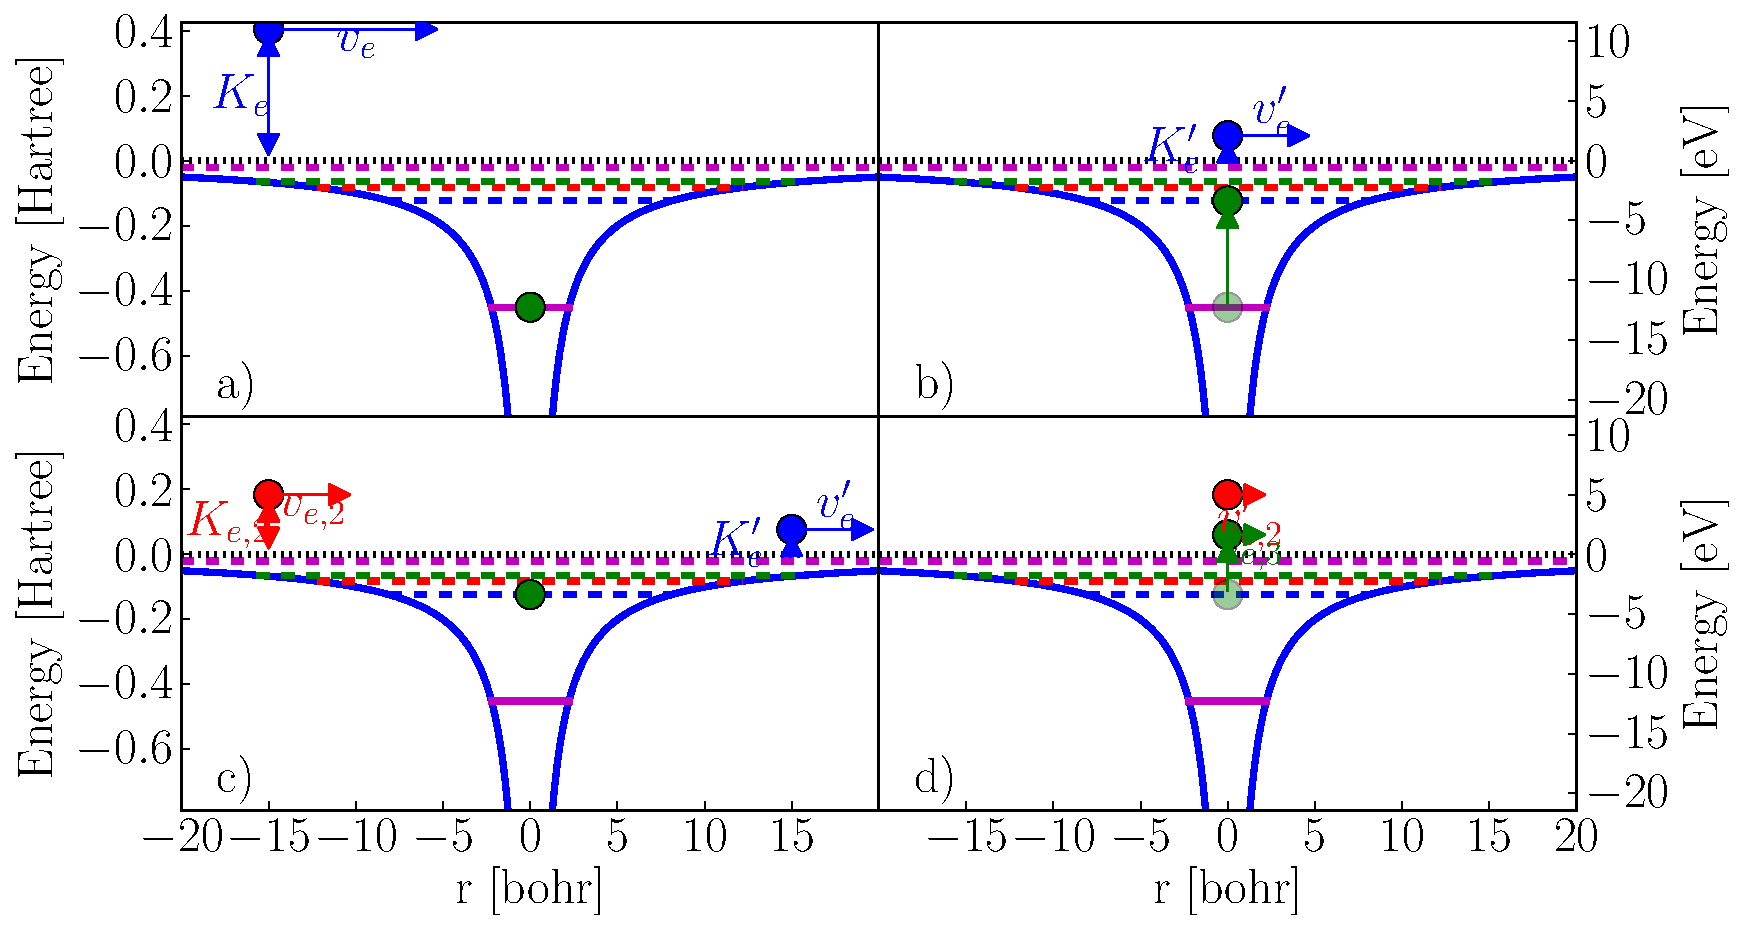
\includegraphics[width=\figurewidth]{figures/ionization_aci}
 \caption{ACI. First electron (in blue) collides with ion in a) and gives
          $K_1$ energy for the transition of a bound electron (in green) to an
          excited state in b).
          A third electron (in red) collides with the ion in c) and
          gives the remaining $K_2$ necessary for the transition to continuum
          in d). The first step is a) to b) and the second step is from c) to d).}
 \label{fig:ionization:aci}
\end{figure}

% \begin{figure}
%  \centering
%     \begin{subfigure}{0.48\columnwidth}
%         \centering
%         \includegraphics[width=\textwidth]{figures/aci_0}
%         \caption{Before}
%         \label{fig:ionization:aci:0}
%     \end{subfigure}
%     \begin{subfigure}{0.48\columnwidth}
%         \centering
%         \includegraphics[width=\textwidth]{figures/aci_1}
%         \caption{1. }
%         \label{fig:ionization:aci:1}
%     \end{subfigure}
% \\
%     \begin{subfigure}{0.48\columnwidth}
%         \centering
%         \includegraphics[width=\textwidth]{figures/aci_2}
%         \caption{2. }
%         \label{fig:ionization:aci:2}
%     \end{subfigure}
%     \begin{subfigure}{0.48\columnwidth}
%         \centering
%         \includegraphics[width=\textwidth]{figures/aci_3}
%         \caption{3. }
%         \label{fig:ionization:aci:3}
%     \end{subfigure}
% \caption{ACI. First electron (in blue) gives $K_1$ energy for the transition
%           to an excited state. Second electron (in green) gives the remaining
%           $K_2$ necessary for the transition to continuum.}
% \label{fig:ionization:aci}
% \end{figure}


Figure \ref{fig:ionization:aci} shows an energy diagram of ACI and the
different transitions possible. This two-step model is implemented using
cross-sections for collisional transition (ground state to excited state and
excited state to continuum), similarly to traditional impact
ionization. See section \ref{section:intro:md:cross-sections} for more
details on cross-sections.

The ACI model revealed to be an important contribution to the field. As will be
seen from the publications, experimental results can be reproduced with this
model.



\subsubsection{Publications}

After the tools are presented in section \ref{section:tools}, the present thesis
consists of a series of four published articles and one article in preparation
where the models and tools are tested and used.


\subsubsubsection{ACI introduction paper}

First, the work on excited states and ACI in clusters was published in the article
``Augmented collisional ionization via excited states in XUV cluster
interactions'' published in 2011 in \textit{Journal of Physics B: Atomic,
Molecular and Optical Physics}\cite{Ackad2011a} and can be found in section
\ref{section:papers:aci} (page \pageref{section:papers:aci}). Argon clusters
(Ar$_{80}$ and Ar$_{147}$) were simulated with parameters used in experiments
at FLASH-DESY in 2008 by Bosted \textit{et al.}\cite{Bostedt2008}.
(32.8 nm -- 37.8 eV, 25 fs and intensities from $\ten{5}{13}$ to
$10^{14}$~W/cm$^{-2}$). It was found that not only ACI could explain the
Ar$^{4+}$ seen at FLASH but also that it
was a dominant process, happening more often than traditional impact ionization.
Due to the efficiency of ACI, high charge states can be reached in shorter time
than previously though which can have a significant impact on biomolecules
imaging. This first ACI article was a stepping stone in the current work as it
showed the validity of the model, as simple as it could be.

\lrfatal{your contributions to this paper.}

\subsubsubsection{Cluster size influence}

Next, section \ref{section:papers:size} presents the article ``Clusters in
intense XUV pulses: Effects of cluster size on expansion dynamics and
ionization''. Also published in 2011 (\textit{Physical Review~A}\cite{Ackad2011b}),
argon clusters were simulated in the XUV regime (32.8 nm,
I~=~$\ten{5}{13}$~W/cm$^{2}$, 25 fs) with cluster sizes from Ar$_{55}$ to
Ar$_{2057}$. It was found that the dynamics is highly collisional and
larger clusters even more so. By rapidly ionizing the lower charge states,
collisional processes will prevent photo-ionization even before the laser pulse
is finished. This mechanism was called \textit{collisionally reduced photoabsorption}.
The amount of energy absorbed through photo-ionization by Ar$_{55}$ clusters was
reduced by 30~\% and 45~\% by Ar$_{2057}$ clusters when collisional processes
are included.
Higher charge states are more abundant and also appears sooner during the
dynamics in large clusters compared to smaller ones. ACI is vital for the
description; 20~\% of ions are in an excited state after the laser peak.
During the laser pulse, the distribution of charge inside clusters is
relatively isotropic but as the simulation evolves, the outer shells tend to
loose electrons more than the core and eventually disintegrate through Coulomb
explosion.
The core stays relatively neutral and expend thermodynamically.

The ion kinetic energy distribution revealed that Ar$^{2+}$  provided most of
the high energy tail. Additionally, the highest charge states had the least
energy. The highest charges states being created in the (neutral) core, the
electrons shield these high charge states, preventing them from accelerating
as much as the outer shells ions.

Electrons thermalize rapidly to a Maxwellian distribution. The larger clusters'
distribution are isotropic due to the high collisional rates while smaller
clusters keep the anisotropy coming from photoionization.


\lrfatal{your contributions to this paper}

\subsubsubsection{Revisiting the 100 nm experiment}
\fxfatal[noinline,margin]{Synchronize and finish the 100nm paper with its description}

Afterwards, section \ref{section:papers:100nm} contains the draft of the article
``Augmented Collisional Ionization in the VUV regime; a theoretical study''.
After Wabnitz \textit{et al.}'s
2002 DESY-FEL experiment's intensity was re-calibrated in 2010, we hypothesized
that our ACI model could still explain the high charge states seen in Xenon
clusters, even with the lower intensities. We included single photon ionization,
impact ionization, ACI and recombination in simulations of Xe$_{90}$ to Xe$_{5083}$
interacting with a 100 fs, 98 nm (12.65 eV) laser pulse at different intensities.
We compared our model
with previous work with ACI disabled and found good agreement. Since these VUV
photons cannot ionize a Xe$^{1+}$ to Xe$^{2+}$ (see table \ref{tab:ips} for Xenon
ionization potentials), all charge states higher than Xe$^{1+}$ must be created
with other processes, in agreement with experiments. The high performance of my
code implementation (see section \ref{section:tools:opencl} on GP-GPU) allowed
running thousands of MD simulations in contrast with other groups where only
a handful of simulations were performed. The chaotic nature of the many-body
problem requires acquiring vast amount of data for valid statistics, giving more
weight to our results. On average, it was found that two more charge states are
accessible when ACI is enabled, a clear indication that ACI has a central role
amongst the ionization channels.

Due to the spacial intensity profile of the laser pulse, simulations were run
at different intensities to simulate the effect of experimental data acquired
from clusters dispersed in the spacial profile. This improves the validity of
simulation data when comparing with experiments. Additionally, our spectrum
was more complete than experiments as they included the neutral Xenon,
inaccessible to the time-of-flight (TOF) apparatus used to collect (real) ions.
Our data was in good agreement with the 2002 experiment. Both the dominant
charge states and the highest charge states matched the experiment data. This
was note the case of other models which used the old intensity.

The last part of the article discuss the influence of the potential depth
of equation~\eqref{eqn:md:sigma}.
% Santra and Greene suggested\cite{Greene2003}
% using atomic potentials instead of a pure Coulombic one to explain the high
% charge states seen in experiments.
By allowing deeper potentials in our
simulations, it was hypothesized that larger charge states could be obtained.
The influence of the potential depth used in simulations is often neglected in
the literature. That article section sheds some light on the topic.
Since electrons are now allowed to go deeper in the ions potential well,
recombination must be used to prevent them from having a total energy less than
the ion's eigenvalues which would not be allowed quantum mechanically.



\subsubsubsection{Recombination }

Finally, section \ref{section:papers:recomb} present the article ``Recombination
effects in soft-x-ray cluster interactions at the xenon giant resonance''
published in May 2013 in New Journal of Physics.

Xenon atoms have, centred at around 13 nm (95.4 eV), a photoabsorption
cross-section approximately ten times larger for the 4d electrons than for the
outer-most shell 5p electrons; inner shell ionization is thus possible and
Auger processes creates highly charged ions, even in the case of xenon
gas\cite{Uiberacker2007}.

In experiments at 13.7 nm (90.5 eV) by Thomas \textit{et al.} in
2009\cite{Thomas2009}, the amount of Xe$^{1+}$ observed in clusters was
significantly more than in xenon gas, indicating that recombination effects were
important. At the time it was clear that photoabsorption and recombination alone
could not explain by itself these results.

Thomas \textit{et al.}'s experiment was described using our models. Xenon
clusters of sizes 147, 1415 and 5083 were simulated under a 13.7 nm
(90.5 eV) laser at different intensities from $\ten{1}{11}$ to
$\ten{5.8}{14}$ W/cm$^2$. Time-of-flight spectra were in good agreement with the
experiment. We also saw that the higher charge states came from the clusters'
outer-shells while the lower charged ions came from the clusters' core. Even
though ions in the neutral core can reach high charge states, they recombine
quickly to lower charge states. The expansion of ionized clusters is best
described by a Coulomb explosion of the outer-shells and a hydrodynamically
expending neutral core.



\subsubsubsection{A quantum approach}

Going further, interesting questions came up. For example, how is a bound
electron's wavefunction affected by a neighbouring ion or the cluster potential?
Due to my background in electromagnetic simulations, I was surprised to read
an article using the FDTD method -- normally used in electrodynamic simulations --
for quantum calculations. I was curious how far could the FDTD method be
applied to quantum problems and if it could answer some of our questions.
A QFDTD simulation package was thus developed, again from scratch,  implementing
two kind of time evolution; real and imaginary. The model and its implementation details
are discussed in section \ref{section:tools:qfdtd}.

The work developed in section \ref{section:tools:qfdtd} was published in the article
``Nonlinear grid mapping applied to an FDTD-based, multi-center 3D
Schr\"odinger equation solver'' presented in section \ref{section:papers:qfdtd}.
Published in 2012 in \textit{Computer Physics Communications}\cite{Bigaouette2011}, it
explains the QFDTD method and its implementation, with emphasis on the new
nonlinear mapping introduced for faster calculation. The QFDTD package is the
first to use both the real and imaginary time evolution, opening the door to
easily get eigenvalues, eigenstates and their time evolution in a time-dependent
and arbitrary spacial shape potential.
The method was first validated by comparing with the analytic solutions of
the hydrogen atom and then applied to solve the H$_{2}^{+}$ molecule.
Comparison with experimental data was in good agreement for the eigenvalues
while the eigenstates could be visualize easily. A new method to calculate
eigenstates is also presented in the article. The publication also
describes in detail the nonlinear mapping that allows reducing both the memory
usage required to store the grid and the time required to calculate the time
evolution. The method is a generic way to obtain a nonuniform grid with cells
concentrated around multi-centres of interest for used in any (finite difference
based) partial differential equation solvers.


% Additionally, section \ref{section:other} specifies other, non-published,
% contributions that were made during the years. The reader will find, in appendix
% \ref{appendix:code}, an overview of the usage of the different simulation
% packages and libraries developed.

Before listing the different publication of the current thesis, the different
methodology and tools used and developed throughout the years will be presented
and discussed.



\subsection{Methodology and Tools}
A large selection of tools exist to study laser-cluster interaction,
differentiating themselves through the amount of approximation taken.

Exact solution of the quantum mechanical system is, most of the time,
intractable. Theoretical investigations thus require some degree of
approximation, a compromise between feasibility and exactitude. On one end of
the spectrum, the most general methods is solving the
Time-Dependent \schrodinger Equation (TDSE) directly or the Quantum Monte-Carlo
(QMC) method. Unfortunately, these methods can only be applied to the simplest
systems of small numbers of electrons; clusters cannot be studied using these
methods.

Larger systems can be studied using \textit{ab initio} methods (``from
first principles'') which covers a wide range of techniques. In this class of
methods one can find \textit{Hartree-Fock} (HF) methods which consist on
approximating the ground state wavefunction by a single Slater determinant.
In HF methods, instantaneous electron-electron Coulomb repulsion is not
included directly in the system's Hamiltonian. Instead, only the average field
resulting from other electrons is used, giving the often used name of
\textit{self-consistent field} methods. Other \textit{ab
initio} methods are the \textit{Post Hartree-Fock} methods where electron
correlation is added. An example is the \textit{Configuration Interaction} (CI)
method. Because of their great accuracy, these methods are restricted to
relatively small systems, generally less then 10 atoms. Full \textit{ab initio}
treatment of clusters is not possible.

Larger systems requires more approximations. \textit{Density Functional Theory}
is an often used method for cluster studies requiring quantum aspects, with
either quantum or semiclassical propagation. It starts by formulating an
expression for the total energy of electrons and ions and derives static and
dynamic equations from it. All approximations are done in the selection of this
(energy) functional. The upper limit on these methods is of practical reasons,
mainly computational power available. On the other side, because the chosen
functional approximate the underlying quantum system, specific quantum effects
might not be included, for example shell effects or tunnelling are neglected.

Because DFT methods are mean field in nature, they cannot account for the large
field fluctuations seen in strong field cluster dynamics.

On the end of the methods spectrum lies the rate equations.






For a detailed review of the different methods, see Ref. \cite{Fennel2010}.





\subsection{Molecular Dynamics (MD)}

Due to the high charge states seen in experiment with clusters the only
practical method to microscopically study the ionization dynamics is
\textit{Molecular Dynamics} (MD) methods where ions and electrons are treated
classically.

In MD, bodies interact directly through classical instantaneous forces. Even
though the method's name contains the term ``molecular'', these forces can be
of any nature; gravitational, van der Waals, Lennard-Jones, electrostatic, etc.
The method numerically integrates Newton's equations of motion, resulting in a
time evolution of the system.

The total force acting on particle $i$ of mass $m_i$ from all other $N$
particles in the system is:
\begin{align}
m_i \va_i & = \vF_i = \sum_{j \ne i} \vF_{j \rightarrow i}
\label{eqn:md:newton}
\end{align}
In the present work, the force between charged particles is the instantaneous
electrostatic Coulomb force:
\begin{align}
\vF_{C,j \rightarrow i}\pa{\vr} & =\frac{k q_i q_j}{r_{ji}^2} \hvr_{ji}.
\label{eqn:md:coulomb:F}
\end{align}
which only depends on the distance between particles. Figure
\ref{fig:md:vectors} shows the vectors definition used throughout this work. We
define particle $i$ the particle we are interested in (for example, the
particle we are calculating the force on), and particle $j$ the particle that
is generating the field or potential that is measured at location $i$. We thus
have:
\begin{align}
\vr_{j} + \vr_{j,i} & = \vr_{i} \\
\vr_{j,i} & = \vr_{i} - \vr_{j}
\end{align}
%       _j
%       /|\
%  r_j /   \ r_ji
%     /    _\/
%    /------>i
%       r_i

% \emptyfig{Vectors definition}{fig:md:vectors}
\begin{figure}
 \centering
 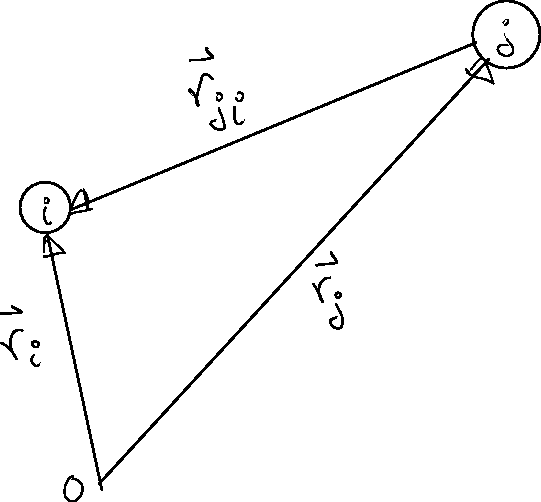
\includegraphics[width=0.38\columnwidth]{figures/mockups/vectors}
 \caption{Vectors definition}
 \label{fig:md:vectors}
\end{figure}


Equation \eqref{eqn:md:newton} can be time integrated using the
Velocity-Verlet (VV) scheme:
\begin{subequations}
\begin{align}
\vx_{i}^{\pa{n+1}} & = \vx_{i}^{\pa{n}} + \vv_{i}^{\pa{n}} \Delta t +
\frac{\va_{i}^{\pa{n}}}{2} \Delta t^2, \\
\va_{i}^{\pa{n+1}} & = \frac{\vF^{\pa{n}}}{m_i} \label{eqn:md:vv:a} \\
\vv_{i}^{\pa{n+1}} & = \vv_{i}^{\pa{n}} + \frac{\va_{i}^{\pa{n}} +
\va_{i}^{\pa{n+1}}}{2} \Delta t,
\end{align}
\label{eqn:md:vv}
\end{subequations}
where $\Delta t$ is the integration time step, $\vx_{i}$ the position vector,
$\vv_{i}$ the velocity vector and $\va_{i}$ the acceleration vector of
particle $i$, all evaluated at either the time step $n$ or the next one $n+1$.
Equations \eqref{eqn:md:vv}, when applied to every particles $i$ of the system,
can thus be used to propagate in time the whole cluster. Note that many
variation of equations \eqref{eqn:md:vv} are possible but all are equivalent.

Every particle in the system stores its position $\vx^{\pa{n}}$, its velocity
$\vv^{\pa{n}}$ and also the total force acting on it $\vF^{\pa{n}}$. This total
force is the sum of all contribution of equation \eqref{eqn:md:coulomb:F} from
all other particles in the system.

The MD algorithm basically calculates the force between every pair of particles
in the system. Since there is $N$ total particles, there is $O\pa{N^2}$
interactions to calculate. Doubling the number of particles will quadruple the
computational burden, effectively putting an upper limit on the number of
particles that can be simulated to tens of thousands.

\subsection{Long range potential: Hierarchical Tree algorithms}
The $O\pa{N^2}$ scaling of MD algorithm can be problematic when the number of
particles simulated is more than many thousands, which is a potential target
for laser-cluster interaction. Some interesting variations of the MD algorithm
exist to reduce the computational burden. These \textit{hierarchical tree}
algorithms were introduced\cite{Barnes1986} by Barnes and Hut in 1986. To
reduce the computational burden, particles are grouped in a hierarchical tree
(quadtree in two dimensions, octree in three). While Barnes used his
\textit{treecode} to solve the N-body problem in the context of gravitational
interactions, it can also be applied in the electrostatic case.

The main issue with the direct calculation of forces in MD is the lack of
distinction between the close particles and distant ones. While the resulting
potential of a distant particle is small, the computational cost required to
calculate it is the same as in the case of a nearby particle. Some MD
calculation use an artificial cutoff; particles farther then this cutoff will
be ignored in the calculation of the force on one particle. This is acceptable
when the force acting on particles is short range, either due to screening or
to the nature of the force. In the present work, the dominant force is the
Coulomb force and is a long range one by nature; it thus cannot be artificially
cutoff as in the case of close range forces used in other fields.

Could distant particles be grouped together, with their contribution to the
force (or potential) being calculated only once (per ``group'')? Because
individual particles which are part of a distant group will have a similar
contribution to the potential at the location of particle $i$, the interaction
with this group can be instead approximated through the multipole
expansion\cite{Gibbon2002} of the group of particles, or cell in terms of the
tree algorithm:
\begin{align}
\phi_i & = \sum_{j~\textrm{cell}} \phi_{j \rightarrow i} = \sum_{j~{\rm cell}}
\frac{k q_j}{r_{ji}} \\
& \approx \frac{M_{c}}{R}
+ \sum_{\alpha} \frac{r_{\alpha} D_{c,\alpha}}{R^3}
+ \frac{1}{2} \sum_{\alpha,\beta} \frac{
        Q_{c,\alpha,\beta} r_{\alpha} r_{\beta}
    }{R^5}
\end{align}
where $M_{c}$, $D_{c,\alpha}$ and $Q_{c,\alpha,\beta}$ are the monopole, dipole
and quadrupole moments of the cell defined as:
\begin{subequations}
\begin{align}
M_{c}           ~~~~& = \sum_{j~\textrm{cell}} q_{j} \\
D_{c,\alpha}      ~~& = \sum_{j~\textrm{cell}} q_{j} r_{j,\alpha} \\
Q_{c,\alpha,\beta}  & = \sum_{j~\textrm{cell}} q_{j} \pa{3 r_{j,\alpha}
r_{j,\beta} - r_{j}^2} \delta_{\alpha,\beta}
\end{align}
\label{eqn:tree:moments}
\end{subequations}
and $R$ is the distance between the cell's centre-of-charge and the
particle of interest $i$.

% \emptyfig{QUAD TREE}{fig:tree:quadtree}
\begin{figure}
 \centering
 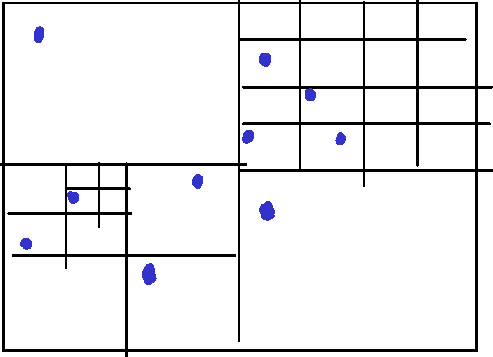
\includegraphics[width=0.38\columnwidth]{figures/mockups/quadtree}
 \caption{Quadtree: 2D's equivalent of the 3D octree}
 \label{fig:tree:quadtree}
\end{figure}

The tree algorithm first split the computational domain into a quadtree until
only a maximum of one particle is present per cell. The tips of the tree,
containing only one particle, are called leaves. Once every particles in the
system are inserted in the tree, the electrostatic moments are propagated from
the leaves up to the root cell, the top cell enclosing the whole domain.

Then, instead of iterating through all particles for the calculation of the
force on the particle of interest $i$, the tree is traversed. If the cell is
``far enough'' (with a given definition of far enough, discussed next) it can
be added to the a cell interaction list for later processing. In the case of
the cell being to close, it must be resolved into its  eight \textit{daughter}
cells. The daughter cells containing particles are visited, while the empty
ones are ignored. The leaf cells can be reached using this process; in this
case, the particles in the leaves are considered close enough to the particle
of interest $i$ and a direct interaction is wanted. The leaf particle will thus
be added to a second interaction list containing particle-particle direct
interactions. The process is recursively repeated until all particles
are added to an interaction list, either directly or through a parent cell.

Different selection rules exist for the criteria of ``far enough''. These
rules are called \textit{Multipole Acceptance Criteria} or
MAC\cite{Pfalzner1996}. Barnes' original one simply referred as
``\textit{s/d}'' compares an input parameter $\theta$ with the cell's size $s$
divided by the distance between the cell's center-of-charge and particle of
interest $i$. If the ratio $s/d$ is smaller than the parameter $\theta$, the
group of particles contained inside the cell is approximated through the cell's
moments and the cell is added to the cells interaction list. At the opposite, if
the ratio is larger than $\theta$, the cell will be resolved into its daughters.
In the limit where $\theta$ reaches zero, no more cells are added to the
cells interaction list (they are all resolved) and the MD algorithm emerges.

Unfortunately, this MAC can cause huge errors when large amount of charge is
present in a corner of a cell. In this case, a cell could be added to the cell
interaction list even though the error introduced by the multipole expansion is
significant. Different MAC have thus been proposed to mitigate this problem.
The \textit{minimum distance} MAC replaces the distance $d$ in the MAC with the
minimum distance to one of the cell's edge. The \textit{B-max} MAC instead
replaces the size of the cell with the largest distance between one of the
cell's corner to the center-of-charge. Another MAC was proposed by Bédorf
\textit{et. al.} \cite{Bedorf2012} and is a mix of the two previous. The MAC
reads:
\begin{align}
d > \frac{s}{\theta} + \delta
\end{align}
where $\delta$ is the distance between the cell's geometric center and its
center-of-charge. If the previous equation holds ($d$ is large enough) then the
multipole expansion is used; the cell is added to the interaction list.

The different MAC can be seen on figure \ref{fig:tree:mac}.

% \emptyfig{MAC DIAGRAM}{fig:tree:mac}
\begin{figure}
 \centering
 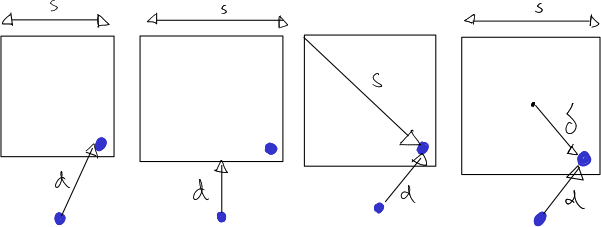
\includegraphics[width=0.8\columnwidth]{figures/mockups/mac}
 \caption{Different Multipole Acceptance Criteria (MAC)}
 \label{fig:tree:mac}
\end{figure}

Because not all interaction pairs are considered in the calculation of the
force and potential, a significant speedup is obtained. Due to the tree
traversal algorithm, the scaling passes\cite{Barnes1986,Gibbon2002,Pfalzner1996}
from $O\pa{N^2}$ to $O\pa{N \ln{N}}$.

A variation to the hierarchical treecode is obtained when a sufficiently large
$\theta$ is used. In this case, the root cell (the largest one) is never
resolved into its daughters. By adding more moments to the approximation then
the first three ones of equations \eqref{eqn:tree:moments} and removing
contributions of nearby particles, the \textit{Fast Multipole Method} (FMM) is
obtained\cite{Pfalzner1996}. FMM was developed by Greegard in
1988\cite{Greengard1987} independently of Barnes' hierarchical tree method.
While conceptually similar, its implementation details are quite different and
has not been implemented in the current work.

\emptyfig{TREECODE SCALING}{fig:tree:scaling}




\subsection{Short range potential: shapes}
\label{section:intro:md:potentials}

An important problem to consider is the close range behaviour of equation
\eqref{eqn:md:coulomb:F} which diverges. Additionally, electrons should not be
able to classically recombine to an ion under the atomic energy level. To
prevent the later, electron recombination, as described in section
\ref{section:intro:clusters:heating}, can be enabled. But this does not prevent
the divergence of the Coulomb force. Instead, the problem is resolved by
changing the shape of equation \eqref{eqn:md:coulomb:F} at close range.
Different \textit{smoothing potentials} can be used to prevent the
discontinuity of the Coulomb potential (or force).


Different potential shapes were investigated for the close range potential.
Figure~\ref{fig:potential:shapes} plots the different shapes of potentials and
their respective electrostatic field. These shapes are obtained by simply
finding the location $R$ where the value and the slope of the close-range shape
$\phi_{cr}$ fits with the Coulomb potential $\phi_C$.
\begin{subequations}
\begin{align}
\left. \phi_C        \right|_{R} & = \left. \phi_{cr} \right|_{R} \\
\left. \delr{\phi_C} \right|_{R} & = \left. \delr{\phi_{cr}} \right|_{R}
\end{align}
\label{eqn:potential:to_match}
\end{subequations}

These locations $R$ are the cutoff radius of these shapes and mark the switch
between the long range Coulomb potential and the short range potential.

\subsubsubsection{Harmonic}
For the harmonic potential, we have:
\begin{align}
\phi_{j,H} & = -A r^2 + \phi_0
\end{align}
We note that at $r_{j,i} = 0$, the potential value is the ``potential depth''
$\phi_0$.
Matching equations \eqref{eqn:potential:to_match} at $R$ gives:
\begin{subequations}
\begin{align}
\phi_{j,H}\pa{\vr_i} & = \frac{-4 \phi_0^3}{27 \pa{k q_j}^2} r_{j,i}^2 + \phi_0
\\
R & = \frac{3 k q_j}{2 \phi_0} \\
\vE_{j,H}\pa{\vr_i} & = \frac{k q_j}{R^3} \vr_{j,i}
\end{align}
\end{subequations}


\subsubsubsection{Super-Gaussian}
The super-gaussian potential is given by:
\begin{align}
\phi_{j,SG}\pa{\vr_i} & = \phi_0 \ex{
                            -\frac{1}{2} \pa{\frac{r_{j,i}}{\sigma}}^{2m}
                        }
\label{eqn:potential:shapes:sg:pot}
\end{align}
In the case where $m = 1$, equation \ref{eqn:potential:shapes:sg:pot} is simply
a gaussian shape. Matching equations \eqref{eqn:potential:to_match} at $R$ gives
values for $\sigma$ and $R$:
\begin{subequations}
\begin{align}
\sigma  & = \frac{k q_j m^{1/2m}}{\phi_0} \ex{\frac{1}{2m}} \\
R       & = \frac{k q_j}{\phi_0} \ex{\frac{1}{2m}} \\
\vE_{j,SG} & = \frac{\phi_0 m}{r_{j,i}}
                \ex{-\frac{1}{2} \pa{\frac{r_{j,i}}{\sigma}}^{2m}}
                \pa{ \frac{r_{j,i}}{\sigma} }^{2m}
                \hvr_{j,i}
\end{align}
\label{eqn:potential:shapes:sg}
\end{subequations}





\subsubsubsection{Gaussian distribution}
An efficient way is to treat electrons as charge distributions instead of point
particles. As such, the electrostatic potential due to a charge particle $j$
(of gaussian shape of width $\sigma$) at location $\vr = r \hvr$ is:
\begin{align}
\phi_{j}\pa{\vr} & = \frac{k q_j}{r} \erf{\frac{r}{\sigma \sqrt{2}}}
\label{eqn:md:smoothed:phi}
\end{align}
The associated electrostatic field is thus:
\begin{align}
\vE_{j}\pa{\vr} & = -\grad{\phi_j\pa{\vr}} = k q_j \pa{
    \frac{ \erf{\frac{r}{\sigma\sqrt{2}}} }{r^2}
    - \sqrt{\frac{2}{\pi}} \frac{ \ex{-\frac{r^2}{2 \sigma^2}} }{\sigma r}
} \hvr
\label{eqn:md:smoothed:E}
\end{align}
When the distance $r$ is large compared to $\sigma$, the error function
is close to 1 and the potential becomes Coulombic. Also, the exponential
term in the electric field will tend towards 0 (since it's a gaussian shape).
The error function will tend towards 1, so the electric field will
be the field of a discrete point charge.

The value of $\sigma$ is arbitrary: the smaller it is, the closer the potential
will be from the pure Coulomb one. We can set a value for $\sigma$ from the
extremum value of the potential which occurs at $\vr = 0$. At $\vr = 0$, an
indetermination $\frac{0}{0}$ occurs. Using l'Hospital rule, we get the limit
of $\phi$ as $\vr$ reaches 0:
\begin{align}
\lim_{\vr \rightarrow 0} \phi_j\pa{\vr}
    & \equiv \phi_j\pa{0} = \frac{ k q_j }{ \sigma } \sqrt{\frac{2}{\pi}}
\end{align}
from which we get the particle width:
\begin{align}
\sigma & = \frac{ k q_j }{ \phi_j\pa{0} } \sqrt{ \frac{2}{\pi}}.
\label{eqn:md:sigma}
\end{align}
The free parameter is thus the ``potential depth'' $\phi_j\pa{0}$. We call this
parameter ``depth'' since the potential energy of an electron on top of an ion
would be minimum, similar to the gravitational potential energy of a ball is
minimum at the bottom of a well.

Another problem that the smoothing of equations \eqref{eqn:md:smoothed:phi} and
\eqref{eqn:md:smoothed:E} solve is the one of \textit{numerical heating} which
occurs when particles artificially gain (or loose) energy during the
calculation of equations \eqref{eqn:md:vv}. This absence of conservation of
energy is due to a time step $\Delta t$ which is too large. Indeed, the
discretization of equations \eqref{eqn:md:vv}, and most importantly of
subequation \eqref{eqn:md:vv:a}, assumes the force on each particle to have a
linear variation between time steps. If the time step is too large and the
curvature of equation \eqref{eqn:md:smoothed:E} can be sampled by the moving
particle between each time steps, then the energy will not be conserved.



Figure \ref{fig:potential:shapes} show the different potential shapes and their
respective electrostatic field.

\begin{figure}
    \begin{center}
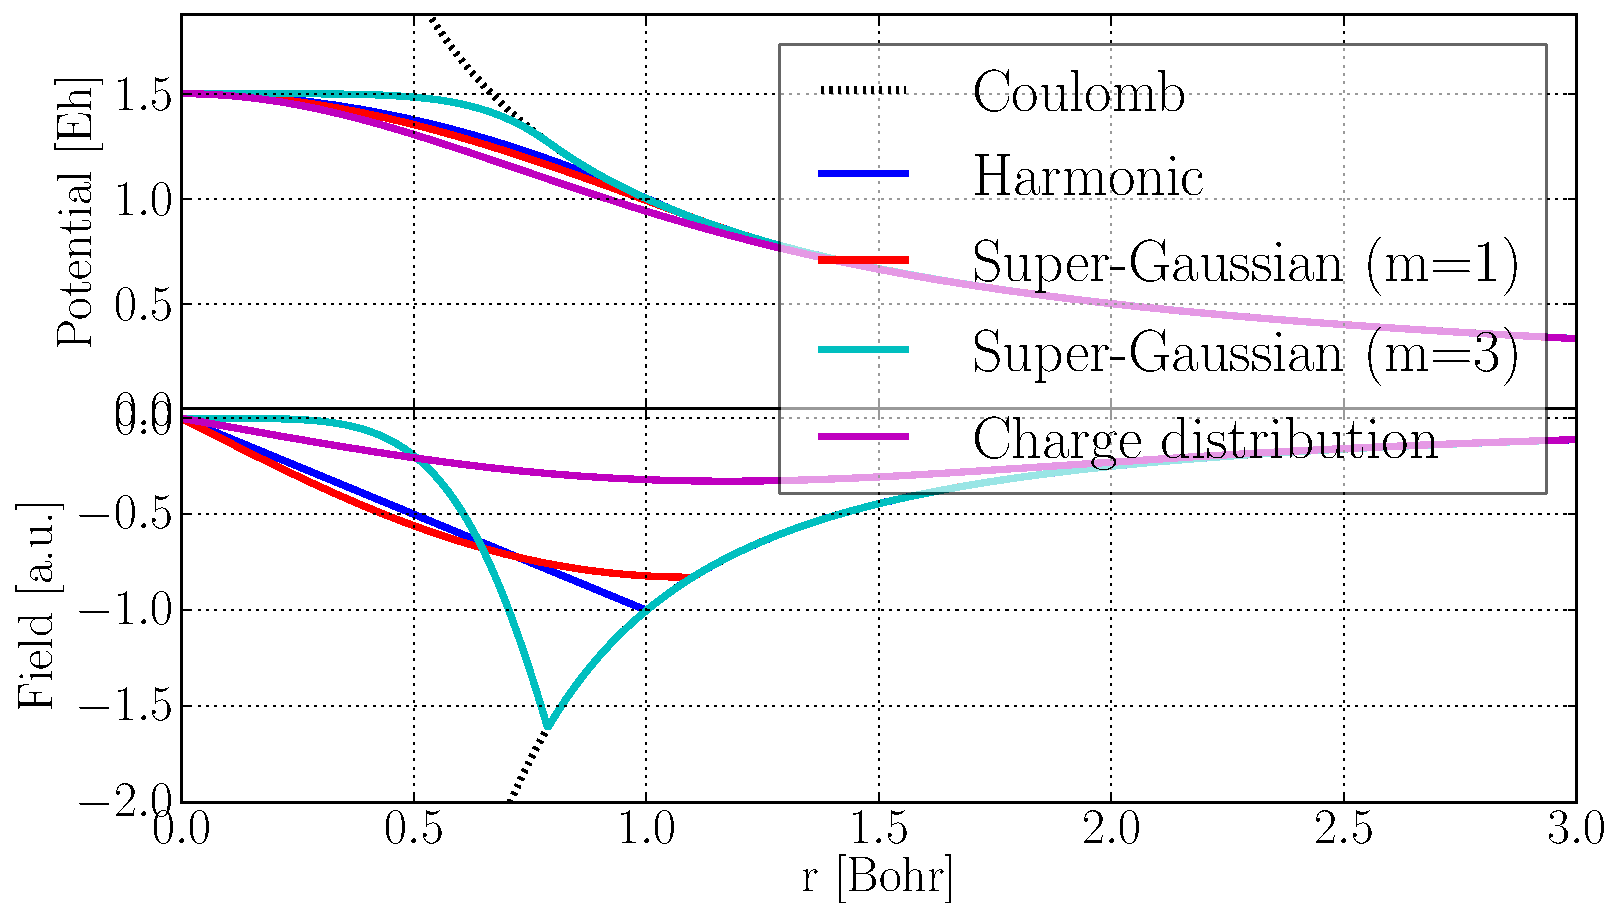
\includegraphics[width=0.98\columnwidth]{figures/potential_shapes}
    \end{center}
    \caption{\label{fig:potential:shapes}Potential shapes and their respective
electric field. Note the use of atomic units and $\phi_0$ = 1.5 Hartree.}
\end{figure}

It was found that the potential given by the charge distribution of equation
\eqref{eqn:md:smoothed:phi} and the associated electrostatic field of
\eqref{eqn:md:smoothed:E} give the less numerical heating. As explained
previously, the time discretization used to integrate the equations of motion
assume that the change in force between two time steps is linear. As can be
seen on figure \ref{fig:potential:shapes}, the charge distribution curve
(magenta) does not have a discontinuity and is therefore the prefered one.

To validate the selection of the smoothing curve, photo-ionization was forced
on a single atom and the total energy tacked. In this ionization case, the
electron comes out of the ion with a maximum of kinetic energy. It is thus a
good candidate to test if numerical heating is present or not. If the total
energy is conserved, then the selected parameters (potential depth, smoothing
curve and time step) can be used with good confidence. Figure
\ref{fig:potential:heating} shows numerical heating.


\emptyfig{NUMERICAL HEATING}{fig:potential:heating}


\subsection{Implementation details}

Our group previously used Barnes and Hut treecode implementation,
freely available\cite{treecode} through the GPL version 2. The code was adapted
to simulate charged particles (Coulomb force) instead of masses (gravitational
force) with some ionization routines added (see for example reference
\cite{Jungreuthmayer2005}). While reducing development time by re-using already
written code, the maintenance burden introduced by many factors (initial
implementation written in the C language, usage of global variables
throughout the code, multiple coding styles from different people throughout
the years, lack of vision, lack of revision control system to give the freedom
of deleting code from the active version without loosing the ability to roll
back, many subtle and important bugs, stability issues, etc.) pushed the author
to restart from scratch. This allowed using modern development techniques to be
used. For example, all development was done through a revision control system
(subversion\cite{svn} at first, then switched to git\cite{git}) in the C++
language instead of C. The object oriented nature of C++ allowed encapsulation
of different parts of the code which could then be tested and validated
individually. This gave better flexibility to the code, a required asset to
push further the development of features.

A substantial number of MD packages are freely available and were
their usage was considered instead of re-implementing a new one from scratch.
Examples are GROMACS\footnote{GROMACS:
\url{http://www.gromacs.org/}}, NAMD\footnote{NAMD:
\url{http://www.ks.uiuc.edu/Research/namd/}} and
LAMMPS\footnote{\url{http://lammps.sandia.gov/}}. A major issue with these
pre-existing MD packages is their target audience; they aim to simulate large
bio-molecules with mostly short range interactions. Another important problem
is the number of particles throughout the simulations; while many packages
assume a constant number of particles, the present work required creating
(ionization) and annihilating (recombination) particles throughout simulations.
Controlling the MD part of the code allowed better integration of the
ionization aspects.

Other MD packages were not mature enough or simply non-existent at the time.
For example the largely used HOOMD-blue\footnote{HOOMD-blue:
\url{http://codeblue.umich.edu/hoomd-blue/}} which uses extensively
Nvidia GPUs released its first version (v0.6.0) in February 2008.
Additionally, the knowledge and experience gained by writing from scratch such
a package is invaluable.

\subsection{Quantum FDTD (QFDTD)}
\label{section:tools:qfdtd}

\begin{itemize}
\item \fxnote{Make sure to state for QFDTD: It's a one electron picture}
\item \fxerror{Add a paragraph or two on mapping as it is NEW.}
\end{itemize}


One model proposed to explain the high charge states seen in some experiments
is the lowering of the ionization barrier, used in conjunction with classical
MD simulations. This model assumes that an electron can be inner ionized when
the potential of a neighbouring ion lowers the potential of the electron's
parent ion. If this barrier is lowered enough so that it drops below the
electron's energy level, the electron becomes free to leave the ion and evolve
in the cluster environment. An open question is how close this model, used
with a classical MD, is to reality. Special care needs to be taken when a
particle, evolving in a quantum world, is to be treated classically. How does
the bound electron's wavefunction reacts to the presence of a second ion
perturbing the potential? How can the $U_b$ approximation to the cluster
environment, described in section \ref{section:intro:Vb}, can be tested?
Is the wavefunction really evolving into a state
where we can say the electron is shared by the two ions? If the electron is
really shared by the two ions, can we classically let it evolve inside the
cluster environment?

These questioned pushed us to look at the quantum aspects in more details. Many
different tools exist to calculate the ground state of a system, even with
multiple electrons, as describe previously. Additionally, excited states are
capital in ACI and as such we wanted a tool that could give us information not
only on the ground state but also on excited states.

After stumbling on an interesting article that used the Finite-Difference
Time-Domain (FDTD) algorithm to solve \schrodinger equation\cite{Sudiarta2007}
it was decided to explore this idea since not much work could be found on this
\textit{Quantum FDTD} (QFDTD) method and due to previous experiences
implementing electrodynamics FDTD.

FDTD is an (old) algorithm developed in 1966 by Yee\cite{Yee1966} to solve
Maxwell's equation on a grid using a leap-frog integration. The number of
scientific articles using FDTD has exponentially increased since the '80s
largely due to the increase in computation resources. Indeed, a three
dimensional grid with the three vector components of both the electric and
magnetic fields requires huge amount of memory that were definitely not present
in the late '60s. The reader is invited to read the excellent book on FDTD by
Allen Taflove and Susan Hagness\cite{Taflove2005} covering 40 years of FDTD
development in electrodynamics simulations.

Other simulation techniques like Finite-Element Methods (FEM) or Finite-Volume
Methods (FVM) can be seen as more complex then Finite-Differences Methods
(FDM). This gives some elegance and simplicity in the FDM algorithms.
Additionally, since FDTD is an explicit algorithm, implementations are
generally easy and efficient and the local nature of the algorithm makes it
easily parallelizable on distributed memory systems.

Sullivan was the first to apply the FDTD method to solve the \schrodinger
equation in his 2000 book\cite{Sullivan2000} where he obtains the wavefunction
of an electron hitting a potential barrier. Latter in 2001 he used the FDTD
method to simulate one and two electrons in a quantum dot\cite{Sullivan2001}.
The Hartree-Fock approximation was used to describe the two electrons problem
and thus required the use of Fourier transforms to calculate the Coulomb
and exchange terms. Due to this extra required calculation, the problem was
restricted to two dimensions only. The following year, he introduced a method
to calculate the eigenstates of an arbitrary system using
FDTD\cite{Sullivan2002}. This method requires two distinct simulations: the
first one finds the eigenvalues and the second one stores the states
corresponding to these eigenvalues, doubling the simulation time required.
The interaction with a magnetic field was included through the vector potential
and later\cite{Sullivan2003,Sullivan2004} used to calculate spin interaction.
Only in 2005 did the first three dimensional
simulations\cite{Sullivan2005a} were performed as proof of concept; only a
single electron was simulated. Eigenstates and eigenvalues were obtained for an
example quantum well as well as a two ions system. A more complicated three
dimensional system was later simulated in \cite{Sullivan2005b}, still with a
single electron.

Later Sudiarta suggested\cite{Sudiarta2007} a new way to use the FDTD method to
solve the \schrodinger equation for a single electron system. By switching to
\textit{imaginary time}, \schrodinger equation can be solved more easily and
more efficiently to get the eigenvalues and eigenstates of the system. It was
later shown that the interaction with a magnetic field could also be added to
the imaginary-time method\cite{Sudiarta2008} and that FDTD could be used to
construct the thermal density matrix of single particle\cite{Sudiarta2009}.

Due to the explicit nature of the FDTD algorithm (values can be obtained at the
next time step from values at the current time step only) the method is
conditionally stable; an upper bound on the time step size must be taken. The
Courant-Friedrichs-Lewy (CFL) condition gives the upper bound. Dai \textit{et
al.} derive\cite{Dai2005} the stability condition for a constant in time
potential:
\begin{align}
\Delta t < \frac{2}{
    \frac{2 \hbar}{m} \pa{
         \frac{1}{\Delta x}
        +\frac{1}{\Delta y}
        +\frac{1}{\Delta z}
        }
        + \textrm{max}\abs{V\pa{\vr}} / \hbar
    }
\end{align}


Both real-time and imaginary-time methods were implemented. Let's describe the
two algorithms.

First, let's define the time dependent \schrodinger equation describing a
wavefunction $\psi$ inside a potential $V$:
\begin{align}
\im \hbar \delt{  } \ket{\psi\pa{\vr, t}}
    & = \pa{-\frac{\hbar^2}{2 m} \laplacian{} + V\pa{\vr, t} } \ket{\psi\pa{\vr,
t}}
\label{eqn:schrodinger:si}
\end{align}
To ease the calculation, let's switch to atomic units where $\hbar = 1$, $m
= 1$ and $e_0 = 1$:
\begin{align}
\im \delt{  } \ket{\psi\pa{\vr, t}}
    & = \pa{-\frac{1}{2} \laplacian{} + V\pa{\vr, t} } \ket{\psi\pa{\vr, t}}
\label{eqn:schrodinger:au}
\end{align}
At initial time $t = 0$, the wavefunction $\ket{\psi\pa{\vr, t}}$ is
decomposed into its eigenstates basis:
\begin{align}
\ket{\psi\pa{\vr, t=0}} & = \sum_{n=0}^{\infty} c_n \ket{\phi_n\pa{\vr}}
\label{eqn:wavefunction:real:initial}
\end{align}
The time-evolution operator (or propagator) $\oU\pa{t}$ is, in atomic units:
\begin{align}
\oU\pa{t} & = \ex{ - \im t \oH }
\label{eqn:propagator:real}
\end{align}
and when applied to the initial state \eqref{eqn:wavefunction:real:initial}
gives the time evolution of the wavefunction:
\begin{align}
\oU\pa{t} \ket{\psi\pa{\vr, t=0}}
    = \ket{\psi\pa{\vr, t}}
  & = \e{ - \im t \oH } \sum_{n=0}^{\infty} c_n \ket{\phi_n\pa{\vr}}
\end{align}
Since the operator $\oH$ applied to the eigenstates
$\ket{\phi_n\pa{\vr}}$ gives the eigenvalues $E_n$, the previous equation
becomes:
\begin{align}
\ket{\psi\pa{\vr, t}}
 & = \sum_{n=0}^{\infty} \e{ - \im t E_n } c_n \ket{\phi_n\pa{\vr}}
\label{eqn:wavefunction:eigenstates:time_evolution:real}
\end{align}
The time evolution of each eigenstates is thus an oscillation between their real
and imaginary parts of which the frequency is given by the eigenvalue $E_n$.



Equation \eqref{eqn:schrodinger:au} can now be solved either in real-time or
imaginary-time, the former being explained first.

Let's separate the real and imaginary components of equation
\eqref{eqn:schrodinger:au} (and simplifying the notation):
\begin{align}
\im \delt{  } \pa{ \psi_R + \im \psi_I}
    & = \pa{-\frac{1}{2} \laplacian{} + V }
        \pa{ \psi_R + \im \psi_I} \\
\im \delt{  } \psi_R - \delt{  } \psi_I
    & = \pa{-\frac{1}{2} \laplacian{} + V } \psi_R
      + \im \pa{-\frac{1}{2} \laplacian{} + V } \psi_I
\end{align}
giving two equations describing the time evolution of two effective fields:
\begin{subequations}
\begin{align}
\delt{  } \psi_R & =   \pa{-\frac{1}{2} \laplacian{} + V } \psi_I
\label{eqn:schrodinger:real:real} \\
\delt{  } \psi_I & = - \pa{-\frac{1}{2} \laplacian{} + V } \psi_R
\label{eqn:schrodinger:real:imag}
\end{align}
\label{eqn:schrodinger:real}
\end{subequations}
The real and imaginary parts in equation \eqref{eqn:schrodinger:real} can be
compared to the electric and magnetic fields in the traditional electrodynamics
FDTD method. The integration is performed using a leap-frog scheme. We
first define $\psi_{i,j,k}^{n}$ the wavefunction located at the grid cell
$\pa{i,j,k}$ and at time step $n$. Then equation equation
\eqref{eqn:schrodinger:real:imag} is evaluated at time step $n$ and, using
(second order) central-differences, we get:
\begin{align}
\left. \delt{  } \psi_I \right|_{n}
& = \left. - \pa{-\frac{1}{2} \laplacian{} + V^{n} } \psi_R \right|_{n} \\
\frac{\psi_{I}^{n+1/2} - \psi_{I}^{n-1/2}}{\Delta t}
& = - \pa{-\frac{1}{2} \laplacian{} + V^{n} } \psi_{R}^{n} \\
\psi_{I}^{n+1/2}
& = \psi_{I}^{n-1/2} - \Delta t \pa{-\frac{1}{2} \laplacian{} + V^{n} }
\psi_{R}^{n}
\label{eqn:schrodinger:real:imag:discretized}
\end{align}
Similarly, defining the time derivative in \eqref{eqn:schrodinger:real:real} at
time step $n$ and again using (second order) central-differences:
\begin{align}
\left. \delt{  } \psi_R \right|_{n+1/2}
& = \left. \pa{-\frac{1}{2} \laplacian{} + V^{n} } \psi_I \right|_{n+1/2} \\
\frac{\psi_{R}^{n+1} - \psi_{R}^{n}}{\Delta t}
& = \pa{-\frac{1}{2} \laplacian{} + V^{n} } \psi_{I}^{n+1/2} \\
\psi_{R}^{n+1}
& = \psi_{R}^{n} + \Delta t \pa{-\frac{1}{2} \laplacian{} + V^{n} }
\psi_{I}^{n+1/2}
\label{eqn:schrodinger:real:real:discretized}
\end{align}

Lastly, the Laplacian is discretized on a grid using (second order)
central-differences:
\begin{align}
\laplacian{} \psi_{i,j,k}^{n} \approx
      \frac{ \psi_{i+1,j,k}^{n} - \psi_{i-1,j,k}^{n} }{2 \Delta x}
    + \frac{ \psi_{i,j+1,k}^{n} - \psi_{i,j-1,k}^{n} }{2 \Delta y}
    + \frac{ \psi_{i,j,k+1}^{n} - \psi_{i,j,k-1}^{n} }{2 \Delta z}
\label{eqn:laplacian:discretized}
\end{align}

Equations \eqref{eqn:schrodinger:real:imag:discretized},
\eqref{eqn:schrodinger:real:real:discretized} and
\eqref{eqn:laplacian:discretized} are then used to propagate in time the real
and imaginary components of the electronic wavefunction. Note that, contrary
to the Yee cell in the electrodynamics FDTD, the two components of the
wavefunction don't have to be defined at different location inside the grid
cell; they are defined at the same location as shown on figure
\ref{fig:qfdtd:cell}.

% \emptyfig{YEE CELL VS QFDTD CELL}{fig:qfdtd:cell}
\begin{figure}
 \centering
 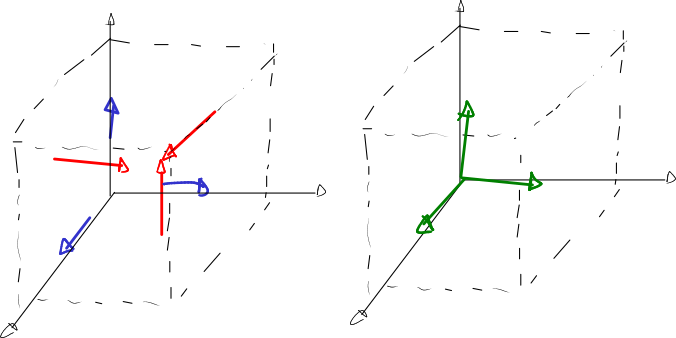
\includegraphics[width=0.8\columnwidth]{figures/mockups/yee_vs_qfdtd}
 \caption{Yee cell used in electrodynamic FDTD vs QFDTD cell
          \fxfatal{$\phi$ is a scalar field!!!}}
 \label{fig:qfdtd:cell}
 \fxwarning[noinline,margin]{Create real figure: Yee cells}
\end{figure}

Equations \eqref{eqn:schrodinger:real:imag:discretized} and
\eqref{eqn:schrodinger:real:real:discretized} by themselves only describe the
time evolution of a wavefunction inside a potential; it does not give a direct
way to obtain the eigenstates of an Hamiltonian. Different approaches exist to
obtain these; Sullivan describes some of them. Eigenvalues though are
relatively easy to obtain though.

By numerically propagating in time a wavefunction $\psi$ using equations
\eqref{eqn:schrodinger:real:imag:discretized} and
\eqref{eqn:schrodinger:real:real:discretized} the system's eigenstates will
evolve according to equation
\eqref{eqn:wavefunction:eigenstates:time_evolution:real}. This evolution is an
oscillation between real and imaginary part at a specific frequency; the states'
eigenvalue. By taking a Fourier transform of the time evolution, eigenvalues
can be identified on a power spectrum. The published article of section
\ref{section:papers:qfdtd} describes a novel method of extracting the
eigenvalues of all eigenstates present in the simulated wavefunction $\psi$.



The second QFDTD method, called the \textit{imaginary-time} method, differs in
that it first requires that the potential be constant in time ($V\pa{\vr, t}
\rightarrow V\pa{\vr}$). Further, a Wick rotation is performed in time ($\im t
\rightarrow \tau$) and the \schrodinger equation in imaginary time is
obtained:
\begin{align}
- \deli{}{\tau} \ket{\psi\pa{\vr, \tau}}
    & = \pa{-\frac{1}{2} \laplacian{} + V\pa{\vr} } \ket{\psi\pa{\vr, \tau}}
\label{eqn:schrodinger:imaginary}
\end{align}
Note that equation \eqref{eqn:schrodinger:imaginary} is not complex and is
similar to the heat equation.


Contrary to the real-time method, the ``time'' evolution of the imaginary
method is not oscillatory. Indeed, the propagator of equation
\eqref{eqn:propagator:real} becomes, in imaginary time:
\begin{align}
\oU\pa{\tau} & = \ex{ - \tau \oH } \label{eqn:propagator:imag}
\end{align}
and the wavefunctions evolution becomes:
\begin{align}
\ket{\psi\pa{\vr, \tau}}
 & = \sum_{n=0}^{\infty} c_n \e{ - \tau E_n } \ket{\phi_n\pa{\vr}}
\end{align}
The imaginary time evolution is thus an exponential growth with the different
eigenstates having different growth rates. It thus becomes possible to isolate
the different eigenstates from each other. A novel method to isolate these
states is described in the published article of section
\ref{section:papers:qfdtd} (page \pageref{section:papers:qfdtd}).

Because equation \eqref{eqn:schrodinger:imaginary} is real, a single scalar
field needs to be discretized on the grid. The discretization is similar to the
real-time method: equation \eqref{eqn:schrodinger:imaginary} is evaluated at
time step $n$ and the time derivative is discretized, in this case using (first
order) forward-differences (and again simplifying the notation):
\begin{align}
- \left. \deli{}{\tau} \psi \right|_{n}
    & = \cro{ \pa{-\frac{1}{2} \laplacian{} + V} \psi }_{n}
\\
\frac{\psi^{n+1} - \psi^{n}}{\Delta \tau}
    & = \pa{\frac{1}{2} \laplacian{} - V} \psi_{n}
\\
\psi^{n+1} & = \cro{1 + \Delta \tau \pa{\frac{1}{2} \laplacian{} - V}} \psi^{n}
\label{eqn:schrodinger:imaginary:discretized}
\end{align}
The Laplacian is discretized with equation \eqref{eqn:laplacian:discretized}.
Since a single scalar field is used to describe $\psi$, special care needs to
be taken in the code implementation. Indeed, equation
\eqref{eqn:schrodinger:imaginary:discretized} uses the Laplacian of the
wavefunction at the previous time step $n$ to update the wavefunction to
time step $n+1$. For example, calculating $\psi^{n+1}_{i,j,k}$ requires
$\psi^{n}_{i-1,j,k}$ and $\psi^{n}_{i+1,j,k}$ (for the $x$ derivative in the
Laplacian) but when calculating the next value in $x$ ($\psi^{n+1}_{i+1,j,k}$)
the required values are now $\psi^{n}_{i,j,k}$ and $\psi^{n}_{i+2,j,k}$, the
former being already updated. The easiest and simplest way to solve this
dependency problem is to store two grids; one for $\psi^{n}$ and another for
$\psi^{n+1}$, alternating between them when calculating equations
\eqref{eqn:schrodinger:real:imag:discretized} and
\eqref{eqn:schrodinger:real:real:discretized}.



\subsection{Acceleration through video cards and OpenCL}
A new trend lately in High Performance Computing (HPC) is code acceleration
through graphics cards. Similar to the ubiquitous Moore's Law in the CPU world,
video cards power evolved exponentially during the last twenty years, pushed
by the never ending need of more realistic video games. From ``dumb'' devices
drawing primitive shapes on a display, they evolved to extremely powerful
devices and started to act more like CPU by being programmable (shaders) during
the first half of 2000. The term \textit{Graphical Processing Unit} (GPU) was
coined in 1999 by Nvidia, the biggest vendor of video cards, as a selling point
to their product and to emphasize the fact that their chips were becoming more
and more alike CPUs.

\subsubsection{General-Programming GPU (GP-GPU)}

Due to this increase in power, people tried to use these video cards as
accelerators for other things than real video operations. Because GPUs have
intrinsically high parallelism (for example the same operation is performed on
all pixels of an image in parallel) HPC users and developers got interested.
In his 2005 book, Taflove described a way to use a video card's GPU to
accelerate his electrodynamics FDTD solver \cite{Taflove2005}. At that time no
General-Programming GPU (GP-GPU) framework existed so Taflove (and anyone
interested in using GPUs at that time) had to ``translate'' the FDTD algorithm
into one that could be understood by a video card. This process was extremely
hard as it required using low level graphic primitives; in his case, OpenGL
calls. Normally OpenGL is used to draw animated scenes on the user's screen.
Notable examples of OpenGL usage is video games where the user is immersed in a
virtual three dimensional space. The process of re-writing an algorithm into
OpenGL calls is one that only a few highly skilled and knowledgeable people can
tackle.

In 2007, Nvidia saw an opportunity for market expansion. Why not let
non-videogames programmer use the powerful GPUs for something else then video
operations? For this to happen, a programming framework had to be released; the
amount of programmers and scientists able to exploit OpenGL to their advantage
was limited. They thus released their \textit{Compute Unified Device
Architecture} (CUDA), later just renamed CUDA. CUDA allows writing normal C or
C++ programs with some extensions, called \textit{kernels}, that can be run on
the GPU. These kernels have the same structure as C functions but are executed
concurrently by every cores on the GPU\footnote{Technically, GPUs don't have
``cores'' \textit{per se} like CPUs but the comparison can still be made.}. The
number of cores on a recent consumer grade video card is now of the order of
many hundreds; a 50\$ Nvidia GT 620 has 96 CUDA cores and 1 GB of RAM, while the
GTX TITAN has 2688 CUDA cores and 6 GB but cost more than 1,000 \$. Even though
the highest priced GPU can be more expensive than complete workstations, no CPUs
can offer close to three thousand cores for a still affordable price.

A year after CUDA was released, Apple wanted a framework that would allow
programs to be accelerated on their top-of-the-line product's GPU while still
being able to run on their lower-end range of products (which did not have a
discrete video card). Additionally, some Apple products were released with ATI
video cards (Nvidia's main competitor) which, understandably, never supported
CUDA. They thus released a framework called \textit{OpenCL} (standing for
Open Compute Language) in 2008 with the help of many partners (IBM, ATI, Intel
and even Nvidia). While conceptually similar to CUDA (smaller routines are
written in a kernel function and launched individually on the GPUs by the main
program) OpenCL has the advantage of targeting heterogeneous platforms
consisting of (possibly and not limited to) many CPUs, many cores and GPUs. The
main advantage of OpenCL is its portability; a program written in OpenCL can
not only run on GPUs from ATI and Nvidia but also on traditional CPUs,
exploiting all cores available on the CPUs transparently.

It was thus decided to port the two codes (MD and QFDTD) to OpenCL to take
advantage of the GPU power while retaining portability.

\subsubsection{GPU programming challenges}
Unfortunately, porting a code to run on GPUs is not as simple as recompiling
for the new architecture. While being portable, OpenCL does requires rewriting
many parts of the code.


\subsubsubsection{Refactoring}
Some things are important to consider when porting codes to GPU frameworks.
First, because a core on a GPU is quite slower than a core on a CPU,
parallelisms must be extracted from algorithms. The code must thus be
completely refactored to exploit the parallelism. For example, a CPU
implementation of the MD algorithm can be implemented by looping over particles
and calculating all properties at once, for every particles. On the contrary,
due to the high vectorized nature of GPUs, it makes more sense to calculate
only one particle property but for all particles before switching to the next
property.

Second, the main drawback of
GP-GPU programming is the fact that GPUs have their own memory, independent of
the system's memory; kernels will only have access to the device's memory. Data
required for kernel calculation must thus be first transferred to the device's
memory and similarly the resulting data must be transferred back to the host
memory where it can be further processed by the rest of the main program. Video
cards today are connected to a computer through PCI-Express (PCIe) connections.
While fast, it can still be a bottleneck if data is to be transferred back and
forth similarly to main memory. It is thus necessary to reduce to a minimum the
data transfer between the host and the device, similarly to communications in a
distributed memory parallel programming paradigm.

In the case of the MD algorithm, every interaction pair is independent of all
others and can thus be calculated concurrently; this is the basis of the
OpenCL implementation. The main loop that calculates the electrostatic field
and potential at every particle's position is implemented as an OpenCL kernel.
Each thread on the GPU will thus calculate the interaction between one particle
and all others. Once the MD kernels are launched on the GPU, they are only
halted when either ionization is to be calculated (every femtosecond) or
when data needs to be saved (to take a snapshot of the simulation for example).
This prevent the GPU from being interrupted too often and reduces the amount of
data transfers. Using this OpenCL implementation, MD simulations could be run
80 times faster than on conventional CPUs.

As for the QFDTD, only the real time algorithm was implemented as OpenCL
kernels since the imaginary time method did not require long simulation times.
As in the case of the MD, the real time algorithm is left running on the GPU
until data needs to be saved to a snapshot or post-processed to reduce
transfers.


\subsubsubsection{Debugging}
One of the most problematic part is the lack of debugging tools. Many different
tools and techniques exist to detect and fix problems in codes.

\subsubsubsubsection{Printing}
The simplest
case is printing the variables' values to the screen and their inspection for
erroneous values. While not really efficient, it is sometimes useful, quick
and simple ``hack'' to get an insight of how the code is working. Unfortunately,
such printing function (such as C or C++'s \textit{printf()}) cannot be used at
all on a GPU! The reason is that the main processor must be able to
\textit{read} the variable from memory to be able to print it to screen and yet
the variable's content is \textit{not} in main memory, only the video card's
memory! It must be noted though that some OpenCL drivers (for example AMD's
APP SDK\footnote{\url{http://developer.amd.com/tools-and-sdks/heterogeneous-computing/amd-accelerated-parallel-processing-app-sdk/}}
or Intel's SDK for OpenCL Applications
2013\footnote{\url{http://software.intel.com/en-us/vcsource/tools/opencl-sdk}})
have specific extensions that allows using \textit{printf()}-like functions
inside OpenCL kernels. These extensions must explicitly be enabled using
\begin{verbatim}
    #pragma OPENCL EXTENSION cl_amd_printf : enable
\end{verbatim}
for the Intel SDK, or
\begin{verbatim}
    #pragma OPENCL EXTENSION cl_intel_printf : enable
\end{verbatim}
for the AMD SDK. These extensions are possible since these drivers support
running the kernels directly on the CPU.

\subsubsubsubsection{Valgrind}
Another useful bug squashing weapon used in debugging on Linux is called
\textit{valgrind}\footnote{\url{http://www.valgrind.org/}}. This extremely
useful tool verifies memory access and can thus report on out-of-bound accesses
(accessing memory locations which are out of range of an array), a major
type of error in programming that one \textit{has} to expect to happen.
Since valgrind was specifically designed to intercept main memory access it
cannot be used when the program is running of a GPU. Alternatively, when the
program is running on the CPU through the use of the Intel or AMD SDKs, valgrind
detects a huge amount of errors, probably due to errors \textit{inside} these
SDKs, rendering the analysis useless.

\subsubsubsubsection{Debuggers}
The last tool used in debugging is an actual debugger. A normal debugger will
take control of the program, allowing the developer to pause the execution
at any time, inspect variables' values or even change them. A popular debugger
on Linux is the free and open-source \textit{gdb}, the GNU Project
debugger\footnote{\url{https://www.gnu.org/software/gdb/}}. Many more
proprietary exists, some of them free and others expensive. Traditional
debuggers, like valgrind, work by taking control of the program and accessing
directly their memory content. It is not possible for them to access GPU memory
or control functions inside the different SDKs. Some debuggers, like
the pricey but powerful DDT\footnote{\url{http://www.allinea.com/products/ddt/}}
allow some form of debugging capabilities on video cards. A free one
called gDEBugger\footnote{\url{http://www.gremedy.com/}} supported
debugging OpenCL kernels. It was acquired by AMD which released an updated
version\footnote{\url{http://developer.amd.com/tools-and-sdks/heterogeneous-computing/amd-gdebugger/}}
in April 2012 but discontinued it. It was superseded by
CodeXL\footnote{\url{http://developer.amd.com/tools-and-sdks/heterogeneous-computing/codexl/}}
released in February 2013. As can be seen, at the time of the code was developed
the different debuggers available were scarce, limited or expensive.


\subsubsubsection{HPC Facilities}
While high performance computing (HPC) are relatively widespread and accessible,
GPU clusters are harder to find.
SHARCNET\footnote{\url{https://www.sharcnet.ca/}}, a large HPC
consortium, has two clusters containing GPUs (Angel and Monk) but they are
obviously submerged by user demand.

\fxnote[noinline,margin]{Is the wording ok?}
Fortunately, a grant was awarded to Professor Paul Corkum of the University of
Ottawa by the Canada Foundation for Innovation's (CFI) Leading Edge Fund and
New Initiatives Fund, of which a percentage was given to both Thomas Brabec
and my supervisor Lora Ramunno for the purchase of a GPU cluster.

Due to my experience with GPUs, I was placed in charge of the purchase process
which consisted in building a solution that would maximize the performance
while staying under-budget, communication with multiple vendors to validate
the solution, writing a Request for Proposals (RFP) and transparently evaluating
vendors offering. Additionally, I (remotely) installed and configured the
operating system (Gentoo Linux\footnote{\url{http://www.gentoo.org/}}) before
the equipment was shipped in August 2012 and also configured the queuing system
(Slurm\footnote{\url{http://www.schedmd.com}}) to maximize the cluster's
resources and even submitting new
features\footnote{\url{http://slurm.schedmd.com/team.html}}.

This HPC cluster, containing 20 Nvidia Tesla M2075 video cards, is an important
lab component that will be allow the research group to continue the high profile
research.



\subsubsection{Close-range: Look-up tables}
\label{section:intro:lut}
The preferred potential shape, the gaussian distribution described in section
\ref{section:intro:md:potentials}, uses the error function which has a major
issue; it is slow, or at least too slow to be called at each interaction pair
calculation. It was decided to move to a look-up table implementation instead.
The potential and field functions are pre-calculated for a charge state of 1+.
Since both potential and field are linear in charge, their value for any
particle is simply scaled by its charge state.

Once the potential and field curves are calculated, they are transferred to the
OpenCL device where they will be indexed using:
\begin{align}
x_{\textrm{norm}} & = \frac{x}{\Delta x} \\
i   & = \textrm{convert\_int\_sat\_rtz}\pa{\textrm{floor}\pa{x_{\textrm{norm}}}} \\
A   &= lut\cro{i} + \pa{lut\cro{i+1}-lut\cro{i}} \pa{x_{\textrm{norm}}-\textrm{convert\_float}\pa{i}}
\end{align}
where $x$ is the distance between the two particles, $lut$ is the array
containing the look-up table, $i$ the index of the look-up table and $A$ the
value to approximate using the look-up table. The OpenCL function
convert\_float() converts an integer to a floating point value
and convert\_int\_sat\_rtz() converts a floating point to an integer,
rounding towards zero (\_rtz) and saturating (\_sat) the conversion in case of
out-of-range
\footnote{\url{https://www.khronos.org/registry/cl/sdk/1.2/docs/man/xhtml/convert_T.html}}
(if the floating point value exceed the range of the integer type,
the maximum value for the integer is used instead of a dangerous undefined
behaviour).

This effectively does a linear interpolation between the look-up table values.
In the present work, 10,000 points are used for the table with a maximum value
for $x$ at the potential shape cutoff distance. In the case of the gaussian
distribution shape, four times the particle width $\sigma$ is used as the cutoff
distance.



\subsubsection{Libraries}

Additionally, a total of seven other libraries were developed to support some
generic features of the code. These libraries are:
\begin{itemize}
\item ionization.git\footnote{ \url{
    https://gitlab.cphoton.science.uottawa.ca/nbigaouette/ionization}}:
    All ionization routines described in section
    \ref{section:intro:clusters:heating}
\item timing.git\footnote{ \url{
    https://gitlab.cphoton.science.uottawa.ca/nbigaouette/timing}}:
    Timing routines used to measure running time, estimated time of arrival
(ETA), etc.
\item stdcout.git\footnote{ \url{
    https://gitlab.cphoton.science.uottawa.ca/nbigaouette/stdcout}}:
    Logging features allowing saving the output of any simulations to a log
    (compressed) file.
\item prng.git\footnote{ \url{
    https://gitlab.cphoton.science.uottawa.ca/nbigaouette/prng}}:
    Pseudo-random number generator (PRNG) library. Wrapper around
dSFMT\cite{prng2009}. Defines easy to use PRNG functions, distributions, seed,
etc. Keeps track of how many times it has been called for easy reloading
exactly where simulation left off.
\item memory.git\footnote{ \url{
    https://gitlab.cphoton.science.uottawa.ca/nbigaouette/memory}}:
    Wrappers around malloc() and calloc() that will automatically check that
    the allocation succeeded. Will also keep track of the amount of
    memory allocated and allow setting a maximum value, preventing
    over-allocation due to bugs or user errors. Can also print values directly
    in binary for easy debugging.
\item io.git\footnote{ \url{
    https://gitlab.cphoton.science.uottawa.ca/nbigaouette/io}}:
    Input and Output library. Wrappers around TinyXML library\cite{tinyxml} for
reading input file. Wrappers around NetCDF\cite{netcdf} for self-contained
output files, used in simulation snapshots.
\item libpotentials.git\footnote{ \url{
    https://gitlab.cphoton.science.uottawa.ca/nbigaouette/libpotentials}}:
    Functions implementing and abstracting different potential shapes.
\item oclutils.git\footnote{ \url{
    https://gitlab.cphoton.science.uottawa.ca/nbigaouette/oclutils}}:
    Library to ease the use of OpenCL devices. Allows selecting the best GPUs
    available on a workstation and locking it to prevent other simulations from
    using it.
\item get\_libraries.git\footnote{ \url{
    https://gitlab.cphoton.science.uottawa.ca/nbigaouette/get_libraries}}:
    Simple script that will download all the previous required libraries,
    compile them and install them in the user's directory.
\end{itemize}
A detailed guide on the compilation and usage of the simulation package can be
read in appendix \ref{appendix:code}.






